\documentclass[sigconf,screen]{acmart}

%%
%% \BibTeX command to typeset BibTeX logo in the docs
\AtBeginDocument{%
  \providecommand\BibTeX{{%
    Bib\TeX}}}

\usepackage{booktabs}
\usepackage{amsmath}
\usepackage{float}
\usepackage[table]{xcolor}
\usepackage{tikz}
\usepackage{microtype}
\usepackage{enumitem}
\usepackage{caption}
\usepackage{stfloats}

% Compact spacing
\setlist{nosep,leftmargin=*}
\captionsetup{font=small,skip=3pt}

\setlength{\textfloatsep}{8pt plus 1pt minus 2pt}
\setlength{\floatsep}{6pt plus 1pt minus 2pt}
\setlength{\intextsep}{6pt plus 1pt minus 2pt}
\setlength{\abovecaptionskip}{3pt}
\setlength{\belowcaptionskip}{2pt}

\setlength{\parskip}{0pt}
\setlength{\parindent}{1em}
\renewcommand{\arraystretch}{1.05}

% Optional ACM compacting for class submission
% Remove these three lines if your professor wants full ACM metadata/copyright block.
\settopmatter{printacmref=false}
\renewcommand\footnotetextcopyrightpermission[1]{}
\pagestyle{plain}

\usetikzlibrary{
  positioning, arrows.meta, calc, fit, backgrounds,
  shapes.geometric, decorations.pathreplacing
}

\definecolor{datablue}{HTML}{4A90D9}
\definecolor{gepagreen}{HTML}{6AB04C}
\definecolor{evalorange}{HTML}{E67E22}
\definecolor{qwkpurple}{HTML}{9B59B6}
\definecolor{trustred}{HTML}{D9534F}
\definecolor{pricegray}{HTML}{95A5A6}
\definecolor{bgblue}{HTML}{EBF5FB}
\definecolor{bggreen}{HTML}{EEF8EA}
\definecolor{bgorange}{HTML}{FEF3E8}
\definecolor{bggray}{HTML}{F4F6F7}

\tikzset{
  B/.style={draw, rounded corners=2pt, minimum height=7mm,
    minimum width=20mm, align=center, font=\scriptsize\sffamily, line width=0.5pt},
  S/.style={draw, rounded corners=1.5pt, minimum height=6mm,
    minimum width=18mm, align=center, font=\tiny\sffamily, line width=0.4pt},
  H/.style={draw, rounded corners=2pt, minimum height=8mm,
    minimum width=22mm, align=center, font=\scriptsize\sffamily\bfseries,
    line width=0.6pt},
  D/.style={draw=black!50, fill=bggray, rounded corners=1.5pt,
    minimum height=6mm, align=center, font=\tiny\sffamily},
  R/.style={draw=trustred, fill=trustred!8, rounded corners=2pt,
    minimum height=7mm, minimum width=20mm, align=center,
    font=\scriptsize\sffamily\bfseries, line width=0.6pt},
  a/.style={-{Stealth[length=1.8mm]}, line width=0.45pt},
  da/.style={-{Stealth[length=1.8mm]}, line width=0.45pt, dashed},
  d/.style={font=\fontsize{5}{6}\selectfont\sffamily, text=black!55},
}

\begin{document}

\title{Optimizing Prompts for Extracting Bitcoin Price Predictions from News Articles}

\author{Bingrui Yang}
\affiliation{
  \institution{Occidental College}
  \city{Los Angeles}
  \state{California}
  \country{USA}
}
\email{byang@oxy.edu}

\author{John Kim}
\affiliation{
  \institution{Occidental College}
  \city{Los Angeles}
  \state{California}
  \country{USA}
}
\email{jkim4@oxy.edu}

\author{Milo Stern}
\affiliation{
  \institution{Occidental College}
  \city{Los Angeles}
  \state{California}
  \country{USA}
}
\email{mstern2@oxy.edu}

\renewcommand{\shortauthors}{Yang, Kim, and Stern}

\begin{abstract}
This study asks whether prompt optimization can help large language models
extract structured Bitcoin price predictions from news articles. We use GEPA
to optimize prompts on 30 manually labeled articles, then evaluate 38 seed and
evolved prompt candidates across four task models on a 35-article held-out
test set. Predictions are mapped to a 1--15 ordinal score that combines
direction and confidence, and are evaluated with parse statistics, exact and
direction accuracy, RMSE, and Quadratic Weighted Kappa (QWK). GEPA produced
longer, more domain-specific prompts, but the selected best prompts did not
consistently outperform the shared seed prompt on test QWK. Across task
models, Claude Sonnet 4.6 achieved the strongest direction agreement, while
Qwen 3.6 achieved the highest combined direction and confidence QWK. These
results suggest that optimized prompting can structure financial news
sentiment, but larger datasets and direction-aware training metrics are needed
for reliable downstream use.
\end{abstract}

\begin{CCSXML}
<ccs2012>
   <concept>
       <concept_id>10010147.10010257.10010293.10010294</concept_id>
       <concept_desc>Computing methodologies~Natural language processing</concept_desc>
       <concept_significance>500</concept_significance>
       </concept>
   <concept>
       <concept_id>10002951.10003317.10003347.10003353</concept_id>
       <concept_desc>Information systems~Sentiment analysis</concept_desc>
       <concept_significance>300</concept_significance>
       </concept>
   <concept>
       <concept_id>10010147.10010257</concept_id>
       <concept_desc>Computing methodologies~Machine learning</concept_desc>
       <concept_significance>300</concept_significance>
       </concept>
</ccs2012>
\end{CCSXML}

\ccsdesc[500]{Computing methodologies~Natural language processing}
\ccsdesc[300]{Information systems~Sentiment analysis}
\ccsdesc[300]{Computing methodologies~Machine learning}

\keywords{prompt optimization, GEPA, financial sentiment, LLM evaluation}

\begin{teaserfigure}
    \centering
    \makebox[\textwidth][c]{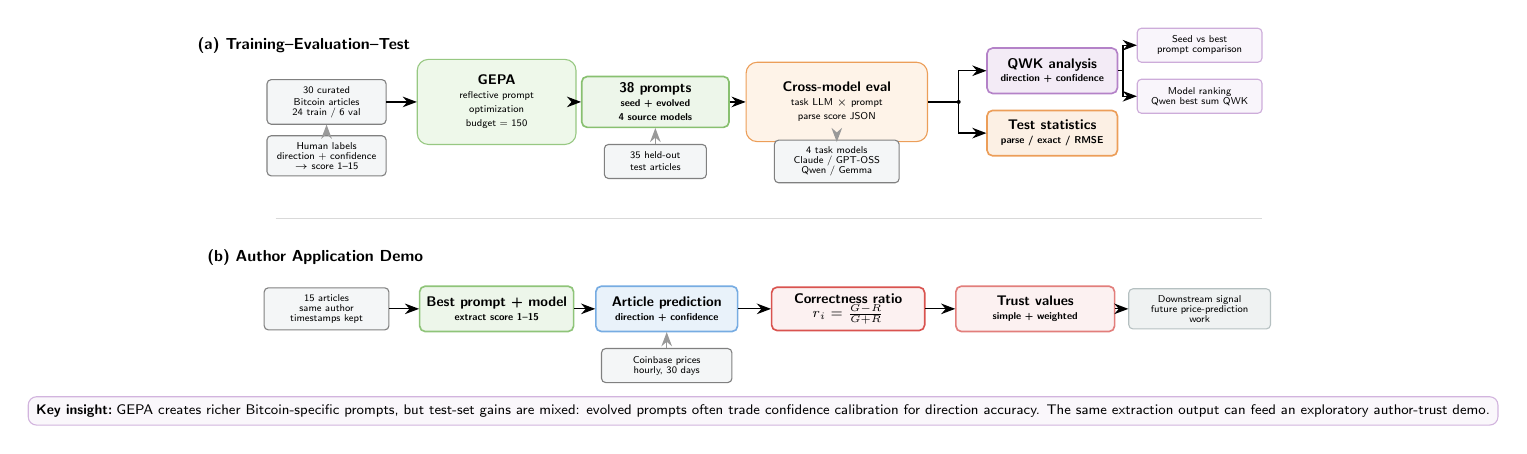
\begin{tikzpicture}[scale=0.72, transform shape]

% ═══════════════════════════════════════════════════════════════
% (a) TRAINING / EVALUATION / TEST — main research workflow
% ═══════════════════════════════════════════════════════════════
\node[font=\footnotesize\sffamily\bfseries] at (-1.2, 1.0)
  {(a) Training--Evaluation--Test};

% Data and labels
\node[D, minimum width=21mm] at (-0.8,0) (train)
  {30 curated\\Bitcoin articles\\[-1pt]{\fontsize{4.5}{5.5}\selectfont 24 train / 6 val}};
\node[D, minimum width=21mm] at (-0.8,-0.95) (gold)
  {Human labels\\[-1pt]{\fontsize{4.5}{5.5}\selectfont direction + confidence}\\[-1pt]
   {\fontsize{4.5}{5.5}\selectfont $\to$ score 1--15}};
\draw[a, black!40] (gold.north) -- (train.south);

% GEPA
\node[draw=gepagreen!70, fill=bggreen, rounded corners=4pt,
      minimum width=28mm, minimum height=15mm,
      align=center, font=\scriptsize\sffamily, inner sep=3pt]
  at (2.2,0) (gepa)
  {\textbf{GEPA}\\[-1pt]
   {\fontsize{5}{6}\selectfont reflective prompt}\\[-1pt]
   {\fontsize{5}{6}\selectfont optimization}\\[-1pt]
   {\fontsize{5}{6}\selectfont budget = 150}};
\draw[a] (train) -- (gepa);

% Prompt pool
\node[H, fill=gepagreen!12, draw=gepagreen!80, minimum width=26mm]
  at (5.0,0) (prompts)
  {38 prompts\\[-1pt]{\fontsize{5}{6}\selectfont seed + evolved}\\[-1pt]
   {\fontsize{5}{6}\selectfont 4 source models}};
\draw[a] (gepa) -- (prompts);

% Test set and task models
\node[D, minimum width=18mm] at (5.0,-1.05) (test)
  {35 held-out\\test articles};
\draw[a, black!40] (test.north) -- (prompts.south);

\node[draw=evalorange!75, fill=bgorange, rounded corners=4pt,
      minimum width=32mm, minimum height=14mm,
      align=center, font=\scriptsize\sffamily, inner sep=3pt]
  at (8.2,0) (eval)
  {\textbf{Cross-model eval}\\[-1pt]
   {\fontsize{5}{6}\selectfont task LLM $\times$ prompt}\\[-1pt]
   {\fontsize{5}{6}\selectfont parse score JSON}};
\draw[a] (prompts) -- (eval);

\node[D, minimum width=22mm] at (8.2,-1.05) (models)
  {4 task models\\[-1pt]{\fontsize{4.5}{5.5}\selectfont Claude / GPT-OSS}\\[-1pt]
   {\fontsize{4.5}{5.5}\selectfont Qwen / Gemma}};
\draw[a, black!40] (models.north) -- (eval.south);

% Metrics
\coordinate (ebr) at (10.35,0);
\draw[line width=0.45pt] (eval.east) -- (ebr);
\fill (ebr) circle (1pt);

\node[H, fill=qwkpurple!12, draw=qwkpurple!75, minimum width=23mm]
  at (12.0,0.55) (qwk)
  {QWK analysis\\[-1pt]{\fontsize{5}{6}\selectfont direction + confidence}};
\draw[a] (ebr) |- (qwk);

\node[H, fill=evalorange!12, draw=evalorange!75, minimum width=23mm]
  at (12.0,-0.55) (stats)
  {Test statistics\\[-1pt]{\fontsize{5}{6}\selectfont parse / exact / RMSE}};
\draw[a] (ebr) |- (stats);

\node[D, minimum width=22mm, fill=qwkpurple!6, draw=qwkpurple!50]
  at (14.6,1.00) (out1)
  {Seed vs best\\[-1pt]{\fontsize{4.5}{5.5}\selectfont prompt comparison}};

\node[D, minimum width=22mm, fill=qwkpurple!6, draw=qwkpurple!50]
  at (14.6,0.10) (out2)
  {Model ranking\\[-1pt]{\fontsize{4.5}{5.5}\selectfont Qwen best sum QWK}};
\coordinate (qwksplit) at (13.25,0.55);
\draw[line width=0.45pt] (qwk.east) -- (qwksplit);
\draw[a] (qwksplit) |- (out1.west);
\draw[a] (qwksplit) |- (out2.west);

% ═══════════════════════════════════════════════════════════════
% DIVIDER
% ═══════════════════════════════════════════════════════════════
\draw[black!15, line width=0.4pt] (-1.7,-2.05) -- (15.7,-2.05);

% ═══════════════════════════════════════════════════════════════
% (b) AUTHOR APPLICATION DEMO — optional downstream validation
% ═══════════════════════════════════════════════════════════════
\node[font=\footnotesize\sffamily\bfseries] at (-1.0, -2.75)
  {(b) Author Application Demo};

\node[D, minimum width=22mm] at (-0.8,-3.65) (auth)
  {15 articles\\[-1pt]{\fontsize{4.5}{5.5}\selectfont same author}\\[-1pt]
   {\fontsize{4.5}{5.5}\selectfont timestamps kept}};

\node[H, fill=gepagreen!12, draw=gepagreen!75, minimum width=24mm]
  at (2.2,-3.65) (best)
  {Best prompt + model\\[-1pt]{\fontsize{5}{6}\selectfont extract score 1--15}};
\draw[a] (auth) -- (best);

\node[H, fill=datablue!12, draw=datablue!75, minimum width=25mm]
  at (5.2,-3.65) (pred)
  {Article prediction\\[-1pt]{\fontsize{5}{6}\selectfont direction + confidence}};
\draw[a] (best) -- (pred);

\node[D, minimum width=23mm] at (5.2,-4.65) (coin)
  {Coinbase prices\\[-1pt]{\fontsize{4.5}{5.5}\selectfont hourly, 30 days}};
\draw[a, black!40] (coin.north) -- (pred.south);

\node[R, minimum width=27mm] at (8.4,-3.65) (ratio)
  {Correctness ratio\\[-1pt]{$r_i=\frac{G-R}{G+R}$}};
\draw[a] (pred) -- (ratio);

\node[H, fill=trustred!8, draw=trustred!75, minimum width=28mm]
  at (11.7,-3.65) (trust)
  {Trust values\\[-1pt]{\fontsize{5}{6}\selectfont simple + weighted}};
\draw[a] (ratio) -- (trust);

\node[D, minimum width=25mm, fill=pricegray!15, draw=pricegray!70]
  at (14.6,-3.65) (future)
  {Downstream signal\\[-1pt]{\fontsize{4.5}{5.5}\selectfont future price-prediction}\\[-1pt]
   {\fontsize{4.5}{5.5}\selectfont work}};
\draw[da] (trust) -- (future);

% ═══════════════════════════════════════════════════════════════
% KEY RESULT / TAKEAWAY — bottom bar
% ═══════════════════════════════════════════════════════════════
\node[draw=qwkpurple!45, fill=qwkpurple!5, rounded corners=3pt,
      minimum width=154mm, align=center, font=\scriptsize\sffamily,
      inner sep=4pt] at (6.9,-5.45) (ins)
  {\textbf{Key insight:}\;GEPA creates richer Bitcoin-specific prompts, but test-set gains are mixed:
   evolved prompts often trade confidence calibration for direction accuracy.
   The same extraction output can feed an exploratory author-trust demo.};

\end{tikzpicture}
}
    \caption{Overview of the Bitcoin news prompt optimization study.}
    \label{fig:teaser}
\end{teaserfigure}

\maketitle

\section{Introduction}

\subsection{Motivation}
Bitcoin (BTC) price coverage is a very nuanced space. The market was born into the digital age, where many traders take to either social media or personal blogs in order to share their sentiments in very informal ways. Many of these predictions take on the form of messy natural language, rather than more traditional finance information tidbits. A single article or post in the BTC space may combine things like analyst quotes, support and resistance levels, macroeconomic contexts, and hedging language. This makes it uniquely difficult to take signals in from the market and make a prediction as to whether an article believes a price is to go up or down in the near future. Furthermore, BTC is one of the most volatile assets on the planet, with sentiment updates and trading occurring around the clock. We want to compare what an article is actually saying versus what later happened in the market.

We were motivated by the desire to turn the signals written into the casual sentiment space into structured data. Instead of asking a model to predict BTC’s price directly, we ask the question of whether an optimized prompt can extract two features from an article published into the space: direction and confidence. Does the author predict a price surge or a tailspin? How confident do they seem in that prediction, and are they hedging their bets? We believe this mechanism creates something more distinctive than a traditional trading algorithm. Instead, we set out to create a careful reader that operates on how the market feels rather than simply how it looks.

Prompt optimization became the clear path because our dataset is small and had to be manually labeled. With such a high cost of harvesting, we skipped model fine-tuning and used GEPA instead. This allows our system to search for a better set of instructions that make LLMs more efficient at producing something as close to the human gold standard as possible. If this approach works, it will suggest that optimized prompting is an efficient way of converting unstructured financial news into analyzable signals. This can later be compared across models, authors, and realized BTC price movements.

\subsection{Research Questions}
Q1: Does GEPA produce prompts that improve structured extraction of
forward-looking Bitcoin sentiment compared with the shared seed prompt? \\
Q2: Which task model best recovers human-labeled direction and confidence on
the held-out Bitcoin news test set?

\subsection{Pipeline Overview}
As shown in Figure~\ref{fig:teaser}, our pipeline first uses GEPA to optimize
prompts on a small manually labeled training set of Bitcoin prediction
articles. We then evaluate all generated prompt candidates across multiple
LLMs on a held-out test set, measuring how closely each model-prompt pair
recovers human gold sentiment scores. Finally, we use the strongest
prompt-model configuration for an optional author-level validation analysis
comparing extracted article predictions with later Bitcoin price movement.

\section{Related Work}

\subsection{Prompt Optimization}
Prompt optimization improves model behavior by modifying instructions rather
than updating model weights. Compared to manual prompt engineering, methods
such as DSPy \cite{khattab2023dspycompilingdeclarativelanguage}, OPRO
\cite{yang2024largelanguagemodelsoptimizers}, and GEPA
\cite{agrawal2026gepa} provide a systematic way to search over prompt
variants. GEPA (Genetic-Pareto) frames this as reflective prompt evolution:
candidate prompts are generated, evaluated on a task metric, and iteratively
refined using feedback from the model's reasoning, while the underlying LLM
remains fixed and is not fine-tuned. This makes GEPA
particularly useful in settings where the goal is to extract reliable
structured outputs without additional model training.

\subsection{LLM Financial Sentiment Analysis}
Financial sentiment analysis uses natural language processing to classify and extract market-relevant signals from an article or post. This is harder than general sentiment analysis as there is market-specific language that is specialized. For example, hedging and bullish vocabulary could mean something completely different out of context. Models such as FinBERT show the value of fine-tuning models for financial text. Their developers show that general sentiment analysis models struggle with domain-specific phrases, along with limited labeled data \cite{araci2019finbert}. More recent work applies larger models to financial documents. Newer LLMs can perform richer extraction tasks that go above and beyond simple binary classification \cite{shen2024financial}. Cryptocurrency sentiment analysis is even more difficult than standard asset price predictions, as it trades continuously. Bitcoin also reacts nearly instantaneously to new information, regardless of the time, as there are no markets that are required to be open to clear trades. Our work aims to build on this literature, but shifts the target from simple predictions to extracting the direction and confidence of predictions embedded in articles.

\section{Method}

\subsection{Models}
We evaluate four Large Language Models (LLMs): Claude Sonnet 4.6,
GPT-OSS-120B, Qwen 3.6, and Gemma 4 (E2B variant). These models were
chosen because they represent the current state of the art across different
model families, offering a wide range of parameter scales and architectural
designs. We used an API key to access Claude and pulled the other three
models from Ollama. LiteLLM was used to call all models through a unified
interface that standardizes interactions with different LLM providers through
a consistent API.

\subsubsection{Claude Sonnet 4.6 (Anthropic)}
This proprietary model is based on a transformer architecture. It incorporates
reinforcement learning from human feedback for alignment and supports
near-instant responses or extended step-by-step thinking, with a 1M-token API
context window in beta \cite{anthropic2026claudesonnet46}.

\subsubsection{GPT-OSS-120B}
This is a transformer mixture-of-experts model from OpenAI with 117 billion
total parameters and a 128K context length, trained on large-scale web and
code data. It is open-weight and designed for local inference
\cite{openai2025gptossmodelcard}.

\subsubsection{Qwen3.6:35b}
This model from Alibaba is trained on multilingual and code-heavy datasets with
a 256K context window. Its distinguishing feature is strong multilingual
capability combined with competitive reasoning performance
\cite{ollama2026qwen36}.

\subsubsection{Gemma 4 (E2B)}
The E2B variant of this open-weight model developed by Google is a relatively
smaller-scale model compared to frontier systems, designed for efficient local
deployment while maintaining reasonable performance. It is trained on a
mixture of web data, code, and curated datasets, with an emphasis on
lightweight reasoning and general language tasks \cite{google2026gemma4e2b}.

\subsection{Data}
The dataset was curated through manual selection from online sources,
specifically filtering for content containing predictive insights rather than
retrospective summaries. This ensures the model learns to identify
forward-looking signals rather than merely processing historical narratives.

To establish a human gold standard, each entry was manually labeled based on
two dimensions: direction and confidence. Direction classifies the nature of
the predicted outcome using a categorical scale of $-1$, $0$, and $+1$, while
confidence represents the certainty expressed by the author on a scale of 1
to 5. These qualitative assessments were then mapped onto a unified 1--15
numerical score, serving as the primary ground truth for training and
evaluating the model's predictive accuracy. Additionally, each entry includes
human-annotated reasoning notes that explain the logic behind the assigned
scores. These notes provide critical context for resolving labeling
ambiguities and serve as a qualitative benchmark for verifying the model's
interpretability during the inference phase.

The dataset is partitioned into three segments for training, evaluation, and
practical application. We used 30 labeled articles for the development phase,
splitting them into 24 for training and 6 for validation, followed by a
separate set of 35 articles for final testing. For the application phase, we
curated 15 unlabeled articles from a single author; these include
high-precision timestamps, which are essential for the longitudinal analysis
discussed later in Section~3.7.

\begin{table}[t]
  \caption{Mapping from direction and confidence to gold score}
  \label{tab:score-mapping}
  \centering
  \scriptsize
  \setlength{\tabcolsep}{2.4pt}
  \renewcommand{\arraystretch}{1.02}
  \begin{tabular}{@{}lccccccccccccccc@{}}
    \toprule
    \textbf{Score} & 1 & 2 & 3 & 4 & 5 & 6 & 7 & 8 & 9 & 10 & 11 & 12 & 13 & 14 & 15 \\
    \midrule
    \textbf{Direction} & $-1$ & $-1$ & $-1$ & $-1$ & $-1$ & 0 & 0 & 0 & 0 & 0 & $+1$ & $+1$ & $+1$ & $+1$ & $+1$ \\
    \textbf{Confidence} & 1 & 2 & 3 & 4 & 5 & 1 & 2 & 3 & 4 & 5 & 1 & 2 & 3 & 4 & 5 \\
    \bottomrule
  \end{tabular}
  \vspace{0.1em}
  \par\raggedright\footnotesize
  For example, a strongly bearish article is labeled direction $-1$ with
  confidence 5, which maps to score 5. A moderately bullish article is labeled
  direction $+1$ with confidence 3, which maps to score 13.
\end{table}

\subsection{Stage 1 --- GEPA Prompt Optimization}
The general optimization objective can be written as:
\begin{equation}
\langle \Pi^*, \Theta^* \rangle_{\Phi}
=
\arg\max_{\langle \Pi,\Theta\rangle_{\Phi}}
\mathbb{E}_{(x,m)\sim T}
\left[
\mu\left(\Phi(x;\langle \Pi,\Theta\rangle_{\Phi}),m\right)
\right].
\end{equation}

This objective searches for prompts that maximize expected task quality. The
term $\mathbb{E}_{(x,m)\sim T}$ averages performance over task instances
sampled from distribution $T$. The operator $\arg\max$ selects the parameter
setting with the highest expected metric score.

\begin{table}[t]
  \caption{Notation for the GEPA optimization framework}
  \label{tab:gepa-notation}
  \centering
  \small
  \setlength{\tabcolsep}{5pt}
  \begin{tabular}{@{}ll@{}}
    \toprule
    \textbf{Symbol} & \textbf{Meaning} \\
    \midrule
    $\Phi$ & Language-model system \\
    $\Pi$ & Collection of prompts \\
    $\Theta$ & Model weights \\
    $x$ & Task input \\
    $m$ & Evaluator metadata \\
    $T$ & Task distribution \\
    $\mu$ & Evaluation metric \\
    $\arg\max$ & Selects the best-scoring parameters \\
    $\mathbb{E}$ & Expected or average performance \\
    \bottomrule
  \end{tabular}
\end{table}

In our implementation, the optimizer is called through
\texttt{gepa.optimize}. For each run, the same source model is used as both
the task model and the reflection model. We initialize the search with a seed
prompt that asks the model to act as a Bitcoin sentiment analyst, consider
only forward-looking claims, ignore retrospective price information, and
return only \texttt{\{"score": <integer 1--15>\}}. For each article, the
evaluator metadata $m$ contains the human gold score and gold reasoning. A
rollout applies one prompt candidate to task examples and compares the model's
JSON score with this metadata.

The metric $\mu$ is the ordinal partial-credit score used by our custom
evaluator. These values become the numeric evaluation signal that GEPA uses to
compare prompt candidates.

\begin{table}[t]
  \caption{Partial-credit evaluator used during GEPA}
  \label{tab:gepa-evaluator}
  \centering
  \small
  \setlength{\tabcolsep}{6pt}
  \begin{tabular}{@{}lc@{}}
    \toprule
    \textbf{Prediction outcome} & \textbf{Score} \\
    \midrule
    Exact match & 1.00 \\
    Off by 1 & 0.75 \\
    Off by 2 & 0.50 \\
    Off by 3 & 0.25 \\
    Off by more than 3 & 0.00 \\
    Parse failure & 0.00 \\
    \bottomrule
  \end{tabular}
\end{table}

The natural-language feedback reports whether the prediction was correct, too
bullish, too bearish, or failed to parse, and it includes the human gold
reasoning as context for reflection. GEPA uses this feedback to revise the
prompt pool by mutating, merging, and selecting candidate prompts according to
evaluated quality.

We set the optimization budget to 150 metric calls for each source-model run.
This budget limits the total number of evaluator calls GEPA can spend across
rollouts, so each iteration must trade off evaluating existing candidates
against exploring revised prompts. We chose this budget as a practical
balance: large enough to allow multiple rounds of prompt evolution, but small
enough to keep the four source-model runs computationally manageable.

This process is executed separately for each of the four source models on the
training dataset, using 24 articles for training and 6 articles for
validation. Across these runs, GEPA produces 38 experimental prompts in total,
including the validation-best prompt selected for each model.

\subsection{Stage 2 --- Cross-Model Test Evaluation}
In Stage 2, every prompt candidate produced in Stage 1 is evaluated with every
task model on the held-out test set of 35 articles. This creates a full
cross-product of 4 task models, 38 prompts, and 35 test articles. For each
prediction, we record the model's parsed score, the gold score, the absolute
and signed errors, parse status, and the ordinal partial-credit score.

\subsection{Stage 3 --- QWK Agreement Analysis}
The 1--15 score should not be treated as fifteen unrelated classes because it
combines two ordinal judgments: direction and confidence. We therefore
evaluate agreement using Quadratic Weighted Kappa (QWK), which accounts for
chance agreement and penalizes larger ordinal disagreements more heavily than
smaller ones. Direction and confidence are evaluated separately, allowing us
to distinguish whether a model fails on the bearish/neutral/bullish boundary
or only on the strength of the prediction.

Let $O_{ij}$ be the observed confusion matrix between gold label $i$ and
predicted label $j$:
\begin{equation}
O_{ij} = \#\{n : y_n = i,\hat{y}_n = j\}.
\end{equation}

The expected matrix under chance agreement is computed from the row and column
marginals:
\begin{equation}
E_{ij} = \frac{r_i c_j}{N},
\end{equation}
where $r_i$ is the number of gold labels in class $i$, $c_j$ is the number of
predictions in class $j$, and $N$ is the total number of parsed predictions.
For $K$ ordinal classes, QWK uses the quadratic weight
\begin{equation}
w_{ij} = \frac{(i-j)^2}{(K-1)^2}.
\end{equation}

The final weighted kappa is then
\begin{equation}
\kappa_w =
1 -
\frac{\sum_{i,j} w_{ij}O_{ij}}
     {\sum_{i,j} w_{ij}E_{ij}}.
\end{equation}

A value of 1 indicates perfect agreement, while 0 indicates chance-level
agreement.

In our case, each 1--15 score is decomposed into direction and confidence:
scores 1--5 are bearish with confidence 1--5, scores 6--10 are neutral with
confidence 1--5, and scores 11--15 are bullish with confidence 1--5. We then
compute QWK once on the three-class direction label and once on the five-class
confidence label. The first analysis compares each GEPA-selected prompt
against its original seed prompt to measure whether prompt optimization
improves agreement. The second analysis aggregates predictions by task model
to compare which model performs best on the rating task. We compare direction
QWK and confidence QWK separately and sum them to obtain the final agreement
score.

\subsection{Author Trustworthiness Evaluation}

To calculate the reliability of an author, we implemented a scoring method that compares the authors market sentiment in an article with Bitcoin movement in the 30 day period after publication. Unlike a binary success/fail evaluation, our method captures both the magnitude and the duration price movements and rewards predictions that is reflected with overall price trends over fluctuations.

\subsubsection{Bitcoin Price Data Collection}

For each article, we record the Bitcoin prices hourly after publication for a month utilizing Coinbase API. The hourly granularity was a limitation of the free tier of the API. The 30-day evaluation window allows sufficient time for the author's prediction to actualize. The window may appear too short in the context of securities at large but it is an overestimate in the context of Bitcoin due to its volatility. An overestimate was done to ensure sufficient data collection.

\subsubsection{Sentiment Score}

15 articles from the same bitcoin author, Manish Chhetri, was fed through Qwen 3.6 model prompted an evolved system prompt from GEPA. The scoring system worked via the following formula:
\begin{equation}
s_i = \Delta + c_i
\end{equation}
where $\Delta$ is a direction-specific offset:
\begin{equation}
\Delta =
\begin{cases}
0 & \text{if bearish} \\
5 & \text{if neutral} \\
10 & \text{if bullish}
\end{cases}
\end{equation}
and $c_i \in [1, 5]$ is the author's expressed confidence in their prediction. This gives three non-overlapping ranges:
\begin{itemize}
    \item Bearish: $s_i \in [1, 5]$
    \item Neutral: $s_i \in [6, 10]$
    \item Bullish: $s_i \in [11, 15]$
\end{itemize}

\subsubsection{Correctness Ratio Classification}

For each hour $(t, t+1)$, we compute the segmented area relative to the baseline $b$ (price at the time of publication) using the trapezoidal rule iteratively updating the calculation. The segment's midpoint is used to assign each as green (correct) or red (incorrect). A simple linear connection between the two price points is a notable limitation of the paper.

For bullish prediction the prediction is correct when the price of bitcoin is above the baseline and incorrect when below. For bear prediction the prediction is correct when the price of bitcoin is below the baseline and incorrect when above.

For neutral predictions, the calculation defines success as price movement within $\pm5\%$ of the bitcoin price at the time of publication, which is a generous window chosen due to bitcoin's volatility.

This partitions the price space into four zones:
\begin{table}[t]
    \centering
    \small
    \setlength{\tabcolsep}{8pt}
    \renewcommand{\arraystretch}{1.15}
    \begin{tabular}{lll}
        \hline
        \textbf{Condition} & \textbf{Label} & \textbf{Classification} \\
        \hline
        $P_t > 1.05 \times P_0$                 & Bullish Escape & Red   \\
        $b \leq P_t \leq 1.05 \times P_0$       & Neutral        & Green \\
        $0.95 \times P_0 \leq P_t < b$          & Neutral        & Green \\
        $P_t < 0.95 \times P_0$                 & Bearish Escape & Red   \\
        \hline
    \end{tabular}
    \caption{Price Zones for a Neutral Prediction}
    \label{tab:zones}
\end{table}

\subsubsection{Correctness Ratio}

The per-article prediction corectness ratio is defined as:
\begin{equation}
r_i = \frac{G - R}{G + R}
\end{equation}

The ratio has several notable properties. The ratio is bounded to $r \in [-1, +1]$. A value of $+1$ indicates that the price was and remained correct for the entire month. A value of $-1$ indicates that the price was and remained incorrect for the entire month. A positive ratio indicates that the author was more right than wrong and vice versa. The data is outputted as a CSV, allowing visualization of how the ratio evolves over the 30-day window.

\subsubsection{Weighted and Unweighted Scores}

Two trust scores are computed with the results.

The simple trust score is the unweighted mean ratio:
\begin{equation}
\tau_{\text{simple}} = \frac{1}{15} \sum_{i=1}^{15} r_i
\end{equation}

The confidence-weighted trust score:
\begin{equation}
\tau_{\text{weighted}} =
\frac{\sum_{i=1}^{15} r_i \cdot c_i}{\sum_{i=1}^{15} c_i}
\end{equation}

The weighted scale is the preferred trustworthiness metric as it penalizes authors who make correct but low-confidence predictions while rewarding those who make bold predictions that prove correct. The denominator $\sum c_i \geq 15$ is always a non-zero value (a positive value) since $c_i \geq 1$.

\subsubsection{Price Movement and PnL Analysis}
 
To further validate the data, we also conducted conventional analyses.
 
The aggregate Bitcoin price movement is calculated for each prediction over the 30-day window. This assesses whether the LLM-extracted sentiment correlates to a price movement in the predicted direction. This serves as a crude check on the scoring system.
 
Profit and Loss (PnL) is also calculated. It charts hypothetical profits and losses in percentage if one bought/shorted bitcoin at \texttt{t = 0} and exited the position at \texttt{t = n}. Neutral articles are excluded from the PnL calculation. Both simple and confidence-weighted aggregate PnL are reported with $\pm1$ standard deviations.
 
A simple timeline is charted to shows the Bitcoin price --- from October 2024 to April 2026 --- with each article's publication date marked. The dot color indicates the predicted direction and the dot size indicates the confidence level. This serves to contextualize the data.

\begin{table}[t]
    \centering
    \small
    \setlength{\tabcolsep}{8pt}
    \renewcommand{\arraystretch}{1.15}
    \begin{tabular}{ll}
        \hline
        \textbf{Condition} & \textbf{Interpretation} \\
        \hline
        $\tau > +0.5$                    & Consistently Correct \\
        $-0.5 \leq \tau \leq +0.5$      & Unreliable or Noisy \\
        $\tau < -0.5$                    & Consistently wrong\\
        \hline
    \end{tabular}
    \caption{Author Trustworthiness Thresholds}
    \label{tab:thresholds}
\end{table}

\section{Results}
 
\subsection{GEPA Prompt Evolution}

\subsubsection{Stage 1 Basic Run Results}

\begin{table}[t]
    \centering
    \small
    \setlength{\tabcolsep}{3pt}
    \renewcommand{\arraystretch}{1.1}
    \begin{tabular}{lrrrrr}
        \hline
        \textbf{Source model} & \textbf{Cand.} & \textbf{Iter.} &
        \textbf{Acc.} & \textbf{Best words} & \textbf{Growth} \\
        \hline
        Claude Sonnet 4.6 & 11 & 15 & 10 & 615 & $6.68\times$ \\
        GPT-OSS 120B & 7 & 20 & 6 & 92 & $1.00\times$ \\
        Qwen 3.6 & 11 & 14 & 10 & 714 & $7.76\times$ \\
        Gemma 4 E2B & 9 & 16 & 8 & 259 & $2.82\times$ \\
        \hline
        \textbf{Total} & \textbf{38} & \textbf{65} & \textbf{34} & -- & -- \\
        \hline
    \end{tabular}
    \caption{Basic Stage 1 GEPA results. ``Best words'' is the word count of
    the GEPA-selected best prompt for that source model, measured against the
    92-word seed prompt.}
    \label{tab:stage1_basic_gepa_results}
\end{table}

Stage 1 optimized prompts separately for the four source models used in the
study: Claude Sonnet 4.6, GPT-OSS 120B, Qwen 3.6, and Gemma 4 E2B. Each run
started from the same 92-word seed prompt and used a budget of 150 evaluator
calls on the 30-article training set. Across the four completed runs, GEPA
retained 38 prompt candidates in the final candidate pools. This total consists
of the four initial seed prompts plus 34 accepted evolved prompts over 65 logged
optimization iterations.

Note: GPT-OSS 120B's GEPA-selected best prompt is the original seed prompt,
which is why its word-count growth is $1.00\times$.

The main change in prompt length was expansion. Three of the four selected
best prompts became substantially longer than the seed: Claude's selected
prompt grew from 92 to 615 words, Qwen's from 92 to 714 words, and Gemma's from
92 to 259 words. GPT-OSS was the exception: although its run generated several
longer prompt candidates, the selected best prompt remained the original
92-word seed. Overall, the Stage 1 results show that GEPA usually preferred
more detailed instructions for this extraction task, but that longer prompts
were not automatically selected in every model-specific run.

\subsubsection{Example Prompt Evolution Tree}

Figure~\ref{fig:claude_prompt_evolution_tree} shows an example GEPA evolution
tree from the Claude Sonnet 4.6 source-model run. The tree visualizes how
accepted prompt candidates branch from earlier prompts rather than following a
single linear revision path.

\begin{figure}[t]
    \centering
    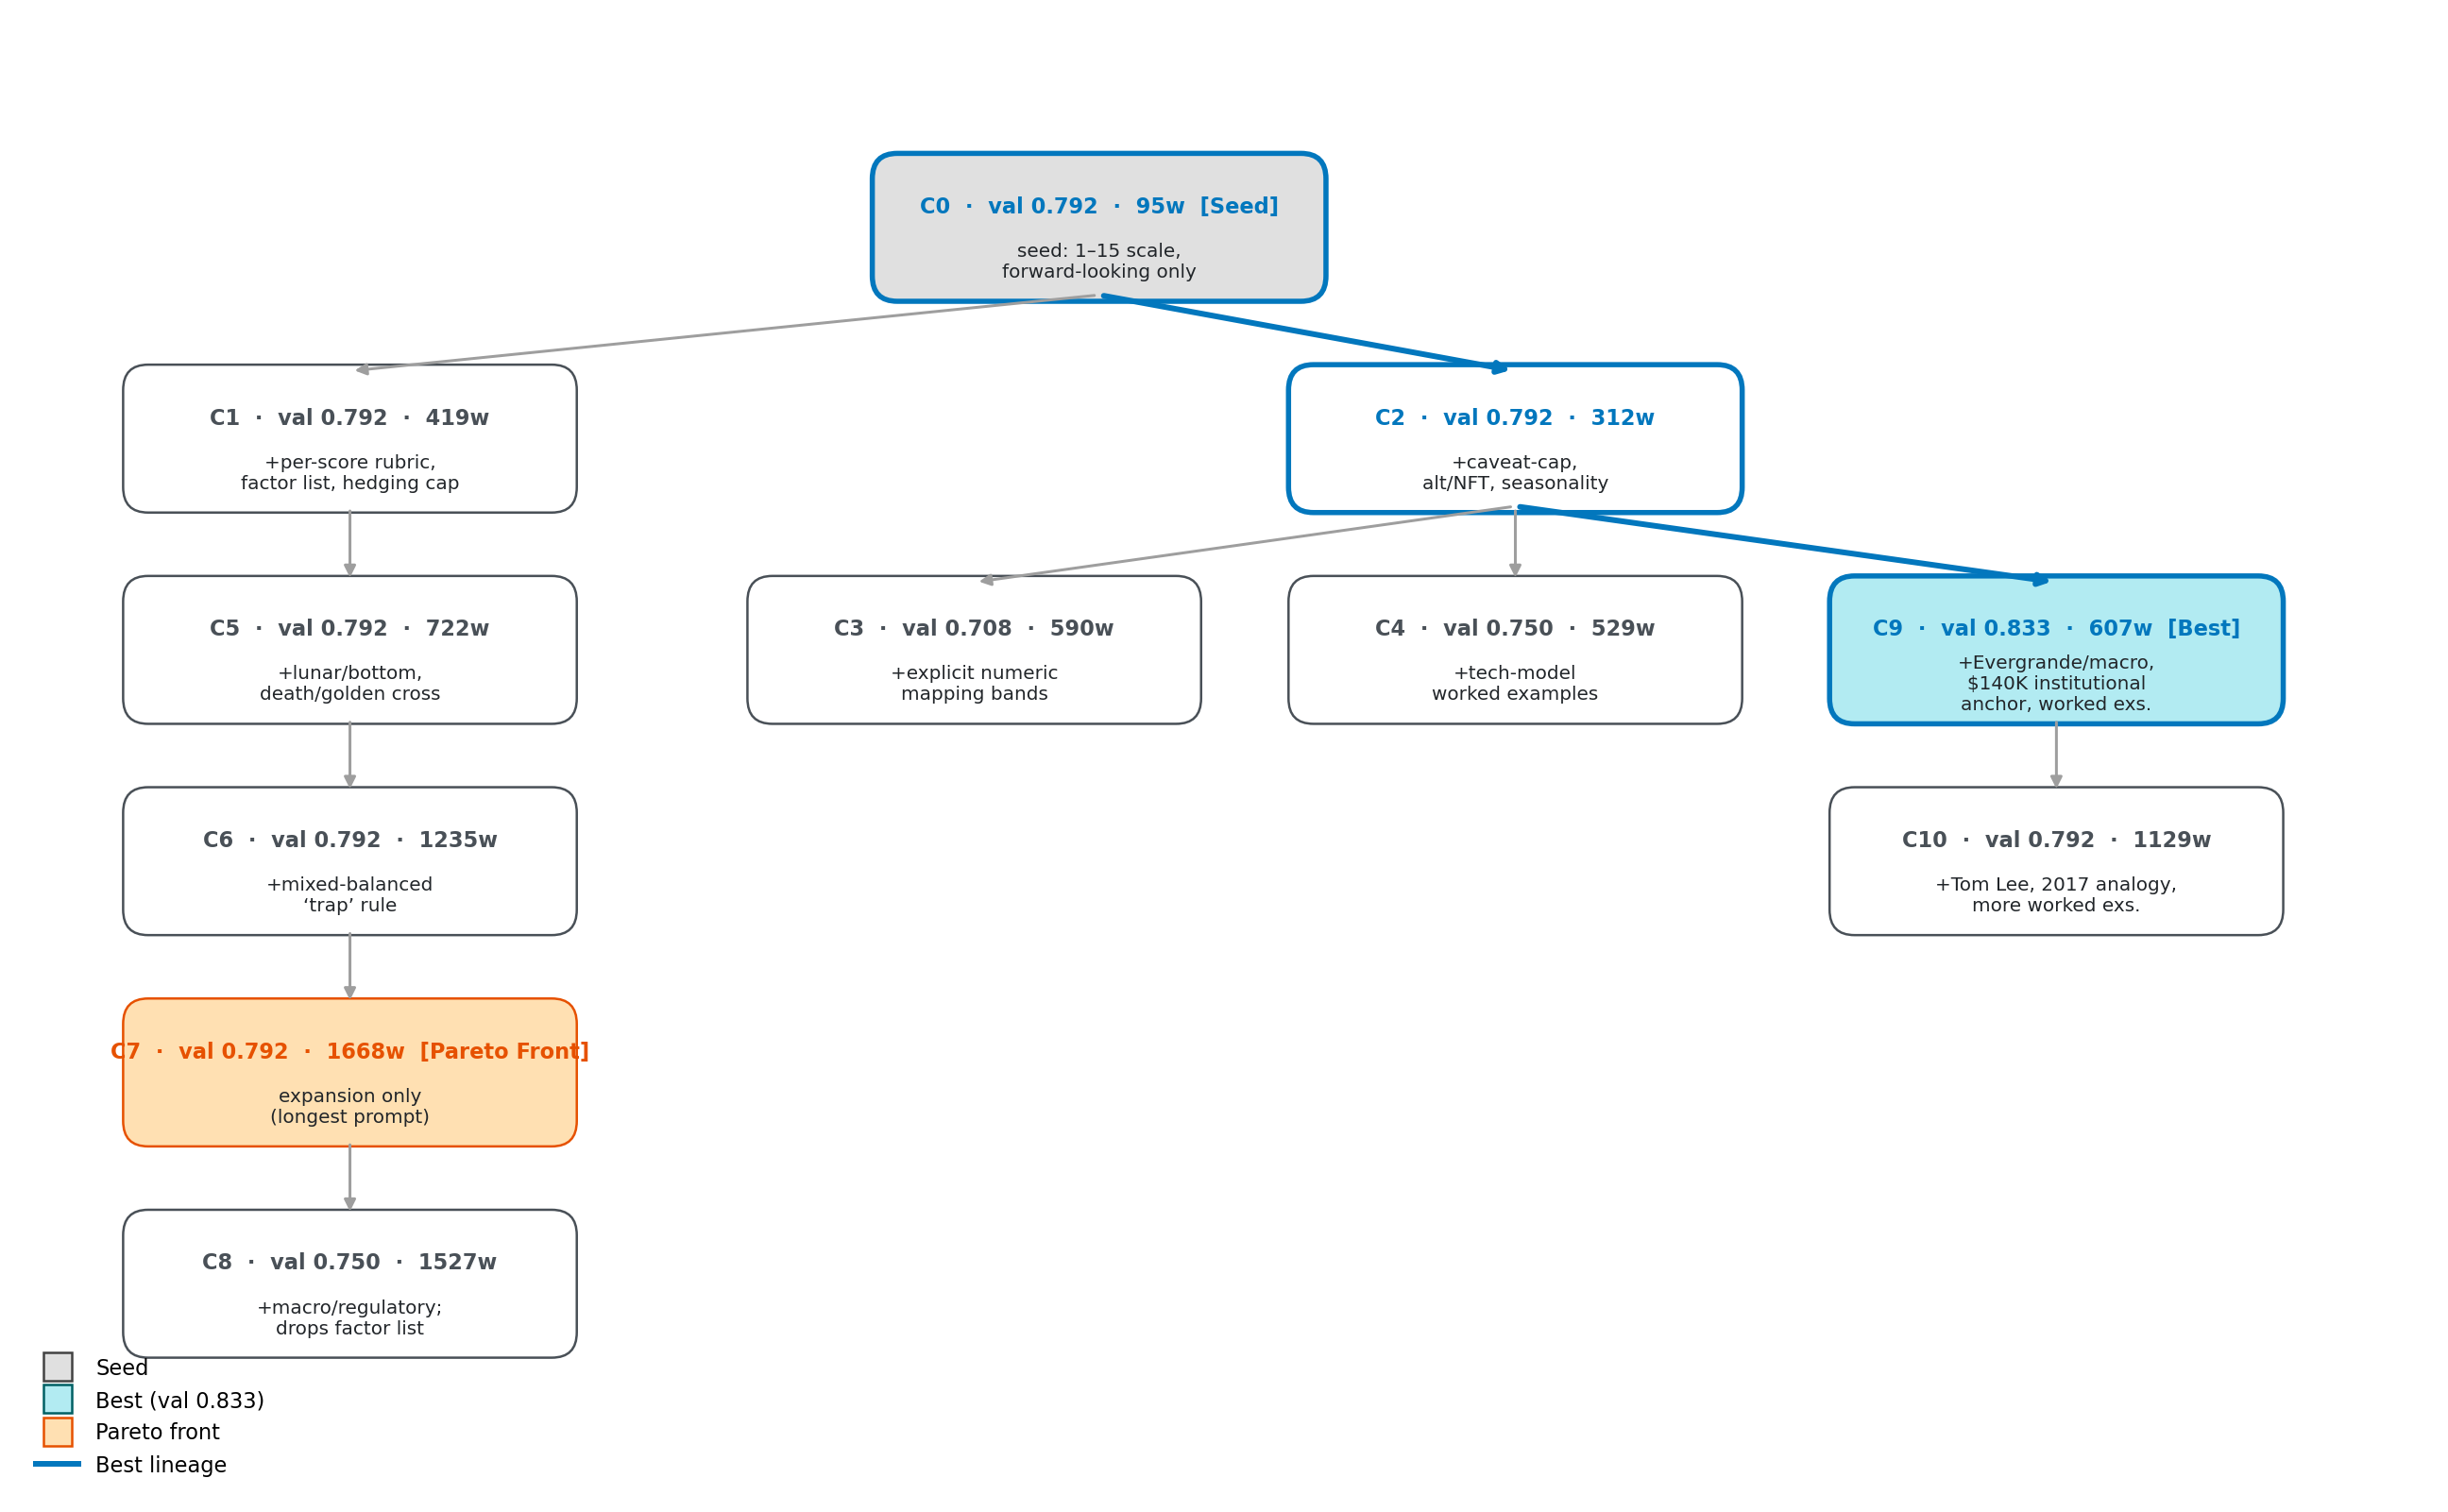
\includegraphics[width=\linewidth]{claude_prompt_evolution_tree.png}
    \caption{Example GEPA prompt evolution tree for the Claude Sonnet 4.6 run.
    Note: C0 is the seed prompt, and the selected best prompt is C9. The best
    path is C0 $\rightarrow$ C2 $\rightarrow$ C9, illustrating that GEPA can
    preserve multiple candidate branches while selecting a later improved
    prompt.}
    \label{fig:claude_prompt_evolution_tree}
\end{figure}

\subsection{Test Evaluation Statistics}

Stage 2 evaluates the prompt candidates produced by GEPA on the held-out
35-article test set. The available test-evaluation artifact contains 4,480
per-article predictions. Claude Sonnet 4.6, GPT-OSS 120B, and Gemma 4 E2B each
have 1,330 predictions, corresponding to 38 prompt candidates evaluated across
35 test articles. The Qwen 3.6 portion contains 490 completed predictions in
the current artifact.

For each task model, we report the parse success rate, exact score accuracy,
direction accuracy, and root mean squared error (RMSE). Parse success measures
whether the model returned a valid structured score. Exact accuracy measures
whether the predicted 1--15 score exactly equals the gold score. Direction
accuracy is less strict: it only checks whether the prediction falls in the
same bearish, neutral, or bullish score band as the gold label. RMSE measures
the typical size of numeric score error after squaring larger mistakes more
heavily. In this setting, it is computed on successfully parsed predictions as
\begin{equation}
\mathrm{RMSE}
=
\sqrt{
\frac{1}{N_{\mathrm{parsed}}}
\sum_{i=1}^{N_{\mathrm{parsed}}}
(\hat{y}_i - y_i)^2
},
\end{equation}
where $\hat{y}_i$ is the predicted 1--15 score, $y_i$ is the human gold score,
and $N_{\mathrm{parsed}}$ is the number of predictions with a valid parsed
score.

\begin{table}[t]
    \centering
    \small
    \setlength{\tabcolsep}{3pt}
    \renewcommand{\arraystretch}{1.1}
    \begin{tabular}{lrrrrr}
        \hline
        \textbf{Task model} & \textbf{Pred.} & \textbf{Parse} &
        \textbf{Exact} & \textbf{Dir.} & \textbf{RMSE} \\
        \hline
        Claude Sonnet 4.6 & 1330 & 81.3\% & 13.0\% & 65.5\% & 2.17 \\
        GPT-OSS 120B & 1330 & 99.6\% & 22.3\% & 77.0\% & 2.85 \\
        Qwen 3.6 & 805 & 82.2\% & 24.6\% & 76.0\% & 2.82 \\
        Gemma 4 E2B & 1330 & 100.0\% & 23.6\% & 67.2\% & 3.57 \\
        \hline
    \end{tabular}
    \caption{Stage 2 descriptive statistics by task model. Exact accuracy and
    direction accuracy are computed over all recorded predictions, so parse
    failures count as incorrect. RMSE is computed only over successfully parsed
    predictions.}
    \label{tab:stage2_test_eval_stats}
\end{table}

The strongest parse reliability appears in the local open-weight models:
Gemma 4 E2B parses every recorded response, and GPT-OSS 120B parses nearly all
responses. GPT-OSS 120B has the highest direction accuracy among the completed
1,330-prediction model runs, while Gemma 4 E2B has the largest RMSE despite
its perfect parse rate. This suggests that valid formatting and numeric
closeness are separate behaviors: a model can reliably produce parseable JSON
while still making larger ordinal score errors.

\subsection{QWK Agreement Results}

\subsubsection{Seed Prompt vs. GEPA-Best Prompt}

The first QWK analysis compares each source model's seed prompt with its
GEPA-selected best prompt under each task model. This creates $4 \times 4 =
16$ task/source comparisons. For each comparison, QWK is computed between the
human gold labels and the model predictions, once for direction and once for
confidence. We also report the sum of the direction and confidence QWK scores
as a combined agreement score.

All source-model runs start from the same seed prompt. Therefore, differences
among seed rows should not be interpreted as differences among distinct seed
prompts. They reflect repeated model calls, retry behavior, parse filtering,
and other run-level variation in the evaluation artifact. Even with this
noise, the table still provides a general comparison between the shared seed
prompt baseline and each source model's GEPA-selected best prompt.

\begin{table*}[t]
    \centering
    \tiny
    \setlength{\tabcolsep}{2pt}
    \renewcommand{\arraystretch}{1.05}
    \begin{tabular}{llrrrrrrrrr}
        \hline
        \textbf{Task} & \textbf{Source} &
        \multicolumn{3}{c}{\textbf{Seed QWK}} &
        \multicolumn{3}{c}{\textbf{Best QWK}} &
        \multicolumn{3}{c}{\textbf{$\Delta$ Best -- Seed}} \\
        \cline{3-5}\cline{6-8}\cline{9-11}
        & & \textbf{Dir.} & \textbf{Conf.} & \textbf{Sum} &
        \textbf{Dir.} & \textbf{Conf.} & \textbf{Sum} &
        \textbf{Dir.} & \textbf{Conf.} & \textbf{Sum} \\
        \hline
        Claude & Claude & 0.908 & 0.254 & 1.162 & 0.912 & 0.049 & 0.961 & 0.003 & -0.204 & -0.201 \\
        Claude & Gemma & \textbf{0.926} & 0.180 & 1.106 & 0.872 & 0.203 & 1.075 & -0.054 & 0.023 & -0.031 \\
        Claude & GPT-OSS & 0.907 & 0.199 & 1.106 & 0.907 & 0.199 & 1.106 & 0.000 & 0.000 & 0.000 \\
        Claude & Qwen & \textbf{0.926} & 0.135 & 1.061 & 0.892 & 0.211 & 1.103 & -0.033 & 0.075 & 0.042 \\
        Gemma & Claude & 0.702 & 0.480 & 1.182 & 0.710 & 0.388 & 1.099 & 0.008 & -0.091 & -0.083 \\
        Gemma & Gemma & 0.789 & 0.329 & 1.117 & 0.792 & 0.453 & 1.245 & 0.004 & 0.124 & 0.128 \\
        Gemma & GPT-OSS & 0.702 & 0.480 & 1.182 & 0.702 & 0.480 & 1.182 & 0.000 & 0.000 & 0.000 \\
        Gemma & Qwen & 0.716 & 0.554 & 1.271 & 0.621 & 0.401 & 1.022 & -0.095 & -0.153 & -0.248 \\
        GPT-OSS & Claude & 0.845 & 0.561 & 1.407 & 0.875 & 0.345 & 1.220 & 0.030 & -0.216 & -0.187 \\
        GPT-OSS & Gemma & 0.774 & 0.580 & 1.353 & 0.816 & 0.313 & 1.129 & 0.043 & -0.267 & -0.224 \\
        GPT-OSS & GPT-OSS & 0.824 & 0.603 & 1.427 & 0.824 & 0.603 & 1.427 & 0.000 & 0.000 & 0.000 \\
        GPT-OSS & Qwen & 0.824 & 0.579 & 1.403 & 0.912 & 0.238 & 1.150 & 0.088 & -0.341 & -0.252 \\
        Qwen & Claude & 0.801 & 0.515 & 1.316 & 0.854 & 0.321 & 1.175 & 0.053 & -0.194 & -0.141 \\
        Qwen & Gemma & -- & -- & -- & -- & -- & -- & -- & -- & -- \\
        Qwen & GPT-OSS & 0.814 & \textbf{0.620} & \textbf{1.433} & 0.814 & \textbf{0.620} & \textbf{1.433} & 0.000 & 0.000 & 0.000 \\
        Qwen & Qwen & 0.814 & 0.587 & 1.401 & -- & -- & -- & -- & -- & -- \\
        \hline
    \end{tabular}
    \caption{Seed-vs-best QWK comparison for all 16 task/source model pairs.
    Direction QWK is computed on bearish, neutral, and bullish labels;
    confidence QWK is computed on the 1--5 confidence label. ``Sum'' is the
    direction QWK plus confidence QWK. Dashes indicate that no parsed rows were
    available for that side of the comparison.}
    \label{tab:qwk_seed_vs_best}
\end{table*}

The seed-vs-best comparison shows that GEPA optimization does not uniformly
increase QWK agreement on the held-out set. Among the 14 comparisons with both
seed and best scores available, the combined QWK score improves in 2 cases, is
unchanged in 4 cases, and decreases in 8 cases. Several best prompts improve
direction agreement while reducing confidence agreement, which suggests that
the optimized prompts can become better at choosing the broad sentiment band
without necessarily improving the finer confidence level inside that band.

\subsubsection{Overall QWK by Task Model}

The second QWK analysis aggregates all parsed Stage 2 predictions by task
model, pooling across source-model prompt candidates and test articles. This
view asks which task model agrees most strongly with the human labels overall,
rather than whether a specific GEPA-best prompt improves over its seed. As in
the first analysis, we report direction QWK, confidence QWK, and their sum.

\begin{table}[t]
    \centering
    \small
    \setlength{\tabcolsep}{3pt}
    \renewcommand{\arraystretch}{1.1}
    \begin{tabular}{lrrrrrr}
        \hline
        \textbf{Task model} & \textbf{Rows} & \textbf{Parsed} &
        \textbf{Parse} & \textbf{Dir. QWK} &
        \textbf{Conf. QWK} & \textbf{Sum} \\
        \hline
        Claude Sonnet 4.6 & 1330 & 1081 & 81.3\% & \textbf{0.873} & 0.137 & 1.010 \\
        Gemma 4 E2B & 1330 & 1330 & 100.0\% & 0.636 & 0.338 & 0.974 \\
        GPT-OSS 120B & 1330 & 1325 & 99.6\% & 0.792 & 0.270 & 1.061 \\
        Qwen 3.6 & 805 & 662 & 82.2\% & 0.794 & \textbf{0.385} & \textbf{1.178} \\
        \hline
    \end{tabular}
    \caption{Overall QWK by task model, computed over all parsed predictions
    available for each model. Rows are all recorded predictions, Parsed is the
    subset used for QWK, and Sum is direction QWK plus confidence QWK.}
    \label{tab:qwk_per_model}
\end{table}

This aggregate view gives a different picture from exact accuracy alone. Claude
Sonnet 4.6 has the strongest direction agreement, but its confidence QWK is
low. Qwen 3.6 has the highest combined QWK score because it pairs competitive
direction agreement with the strongest confidence agreement. Gemma 4 E2B has
perfect parse coverage but the lowest combined QWK, again showing that
formatting reliability and label agreement are not the same behavior.

\subsection{Author Evaluations}

\begin{figure*}[t]
    \centering
    \begin{minipage}{0.48\textwidth}
        \centering
        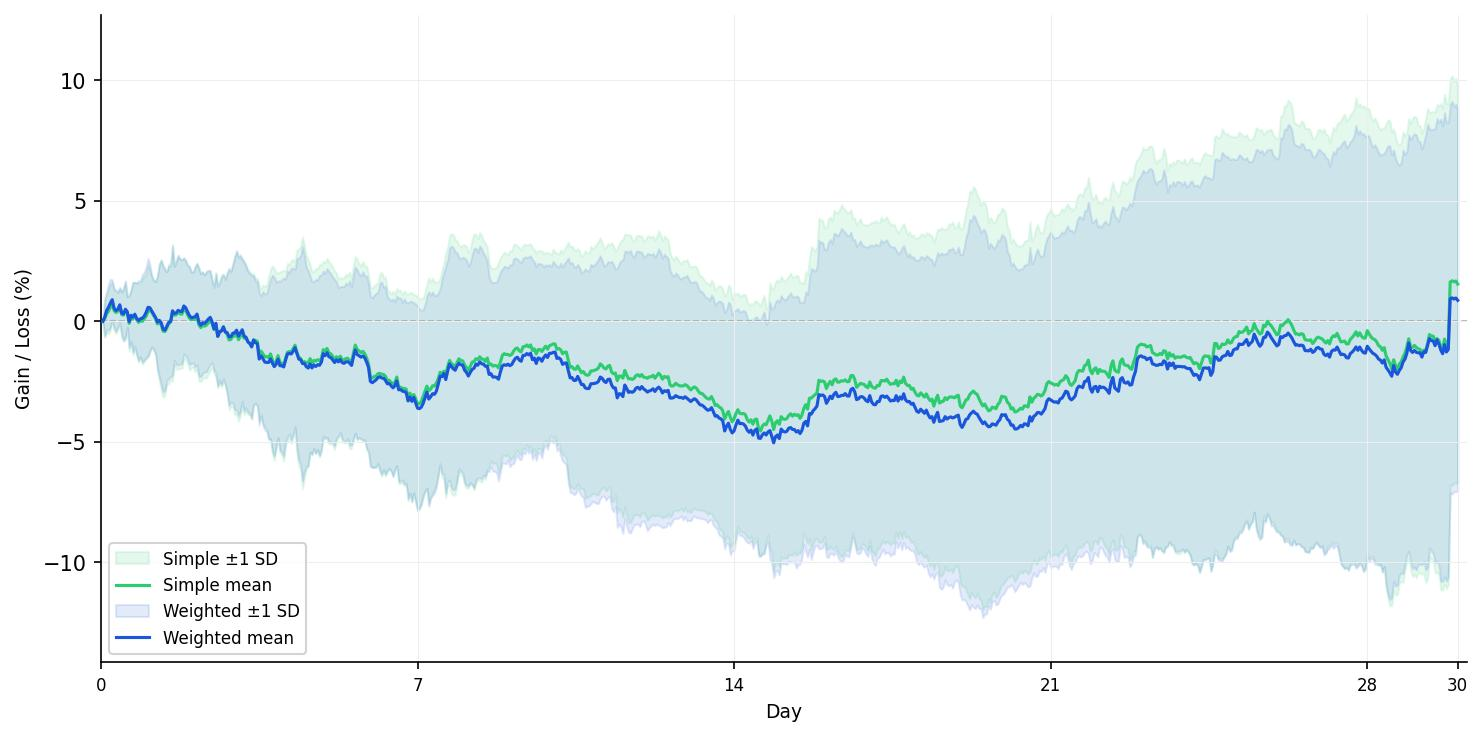
\includegraphics[width=\linewidth]{chart_30day_long_aggregate}
        \caption{30-Day Long Position PnL on Bullish Predictions}
        \label{fig:long_agg}
    \end{minipage}
    \hfill
    \begin{minipage}{0.48\textwidth}
        \centering
        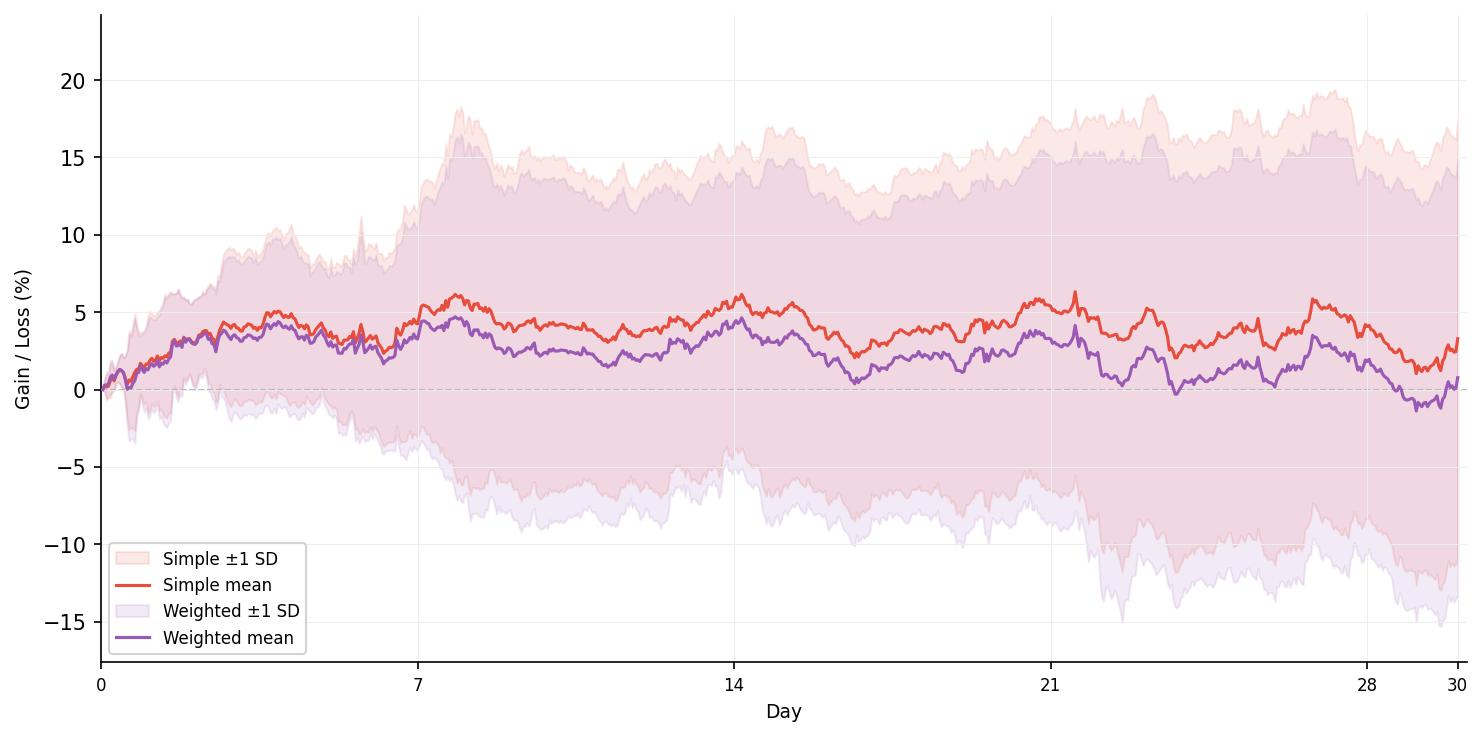
\includegraphics[width=\linewidth]{chart_30day_short_aggregate}
        \caption{30-Day Short Position PnL on Bearish Predictions}
        \label{fig:short_agg}
    \end{minipage}

    \vspace{0.4cm}

    \begin{minipage}{0.48\textwidth}
        \centering
        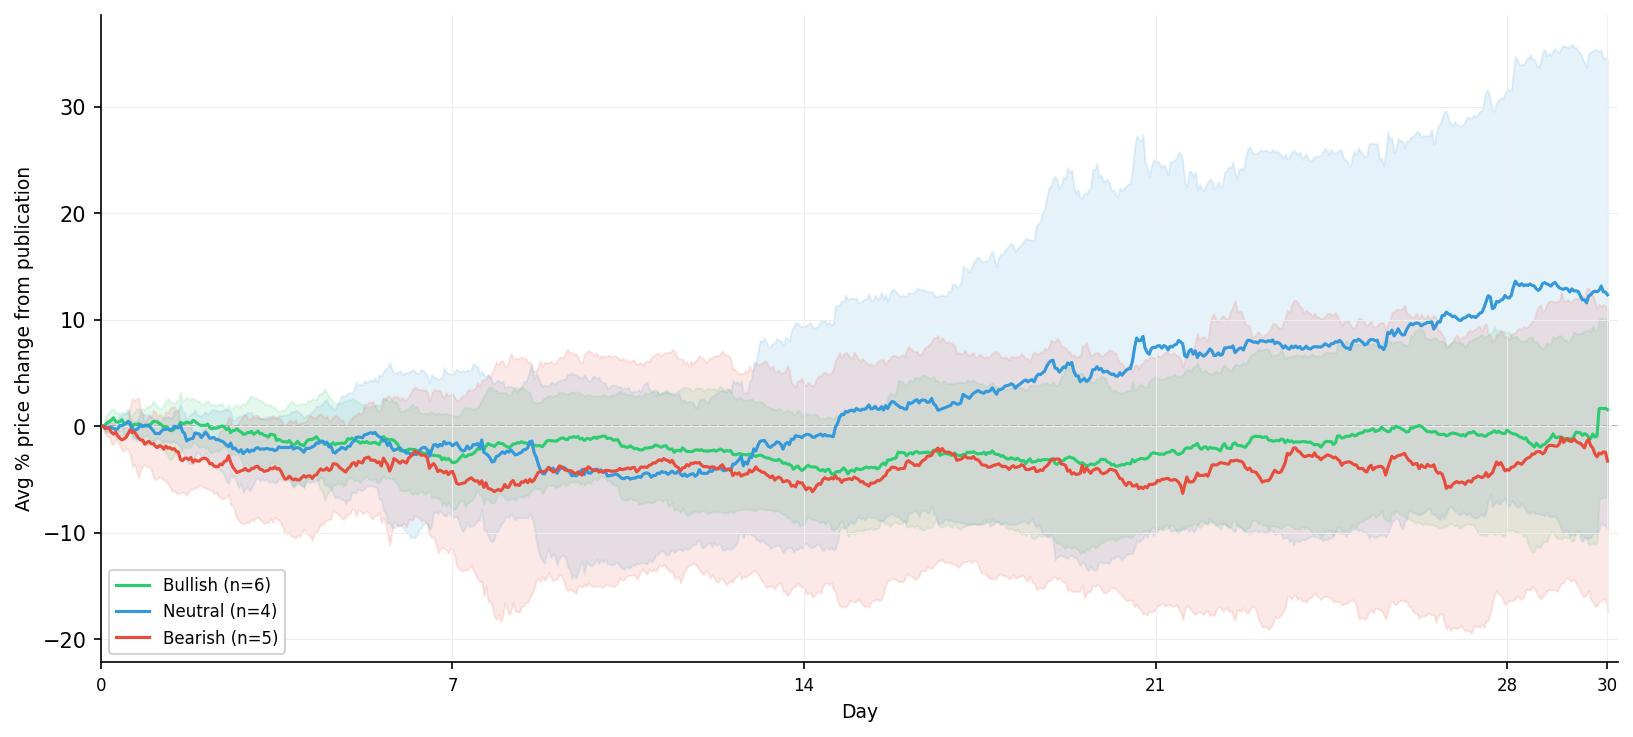
\includegraphics[width=\linewidth]{chart_btc_movement_by_direction(1)}
        \caption{Bitcoin Price Movement by Predicted Direction}
        \label{fig:btc_movement}
    \end{minipage}
    \hfill
    \begin{minipage}{0.48\textwidth}
        \centering
        
\includegraphics[width=\linewidth]{BTC_Price_Sentiment_Prediction/chart_ratio_by_direction(1).jpg}
        \caption{Trust Ratios}
        \label{fig:agg_ratio}
    \end{minipage}

    \vspace{0.4cm}

    \begin{minipage}{\textwidth}
        \centering
        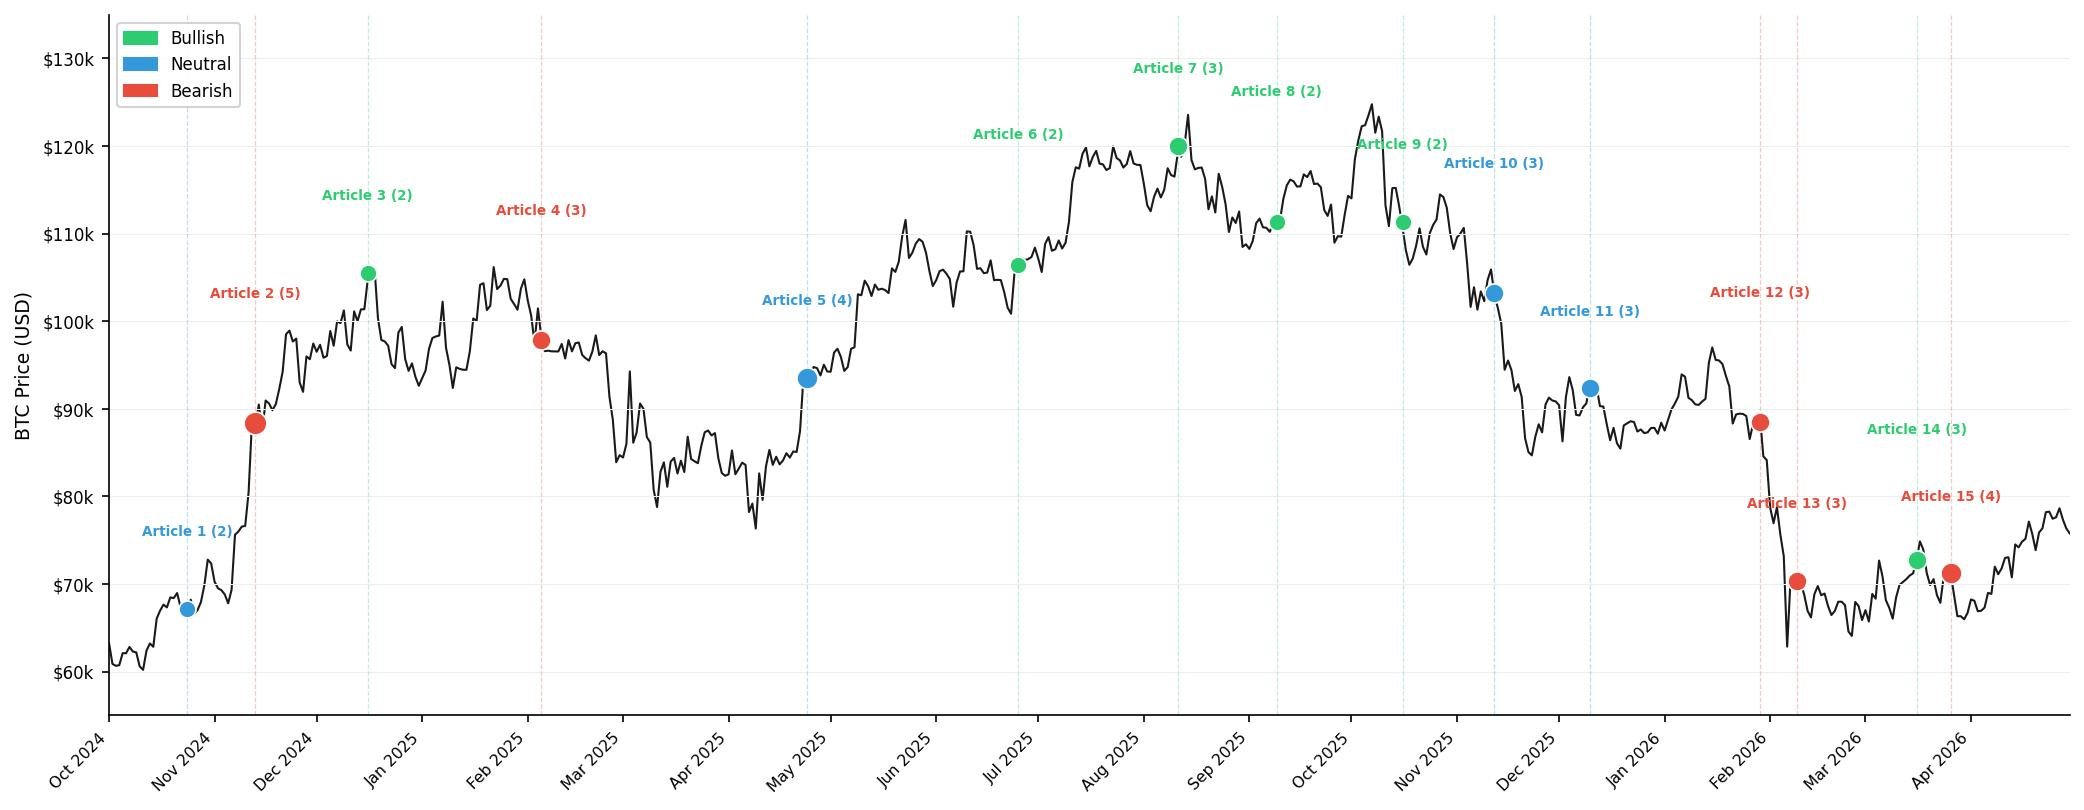
\includegraphics[width=\linewidth]{chart_btc_at_publication}
        \caption{Bitcoin Price Movement Compared Against Article Publication with Confidence Scores}
        \label{fig:btc_at_publication}
    \end{minipage}
\end{figure*}

Figure~\ref{fig:btc_at_publication} shows the Bitcoin price movement compared to the 15 articles with prediction and confidence. The author published predominantly bullish articles especially during the mid-2025 price peak (articles 6--9), and shifted toward bearish calls (articles 12--15) as the price tumbled. The clustering suggests the author is reacting to the market rather than predicting it.
 
Figure~\ref{fig:agg_ratio} shows the aggregate running ratio in the 30-day window. The simple and weighted trust scores begin positive at publication and peaks at the 12 hour mark and maintains above 0.5 for the first 72 hours. It then steadily decreased and crosses zero around day 23.
 
Figure~\ref{fig:btc_movement} shows the aggregate Bitcoin price movement by predicted direction. Bearish articles show a consistently strong sustained price movement in the predicted negative direction. However, bullish and neutral predictions are much more inconsistent. In fact, the neutral price outperforms the bullish by the week 2 mark. But this can be attributed to the limited sample size of 15 articles. 
 
Figures~\ref{fig:long_agg} and~\ref{fig:short_agg} show the simulated 30-day PnL for long and short positions respectively. Long positions on bullish articles consistently shows a negative PnL (loss), reflecting the limited bullish performance. Short positions on bearish articles, however, shows a consistently positive PnL (profit) throughout.

\section{Discussion}

\subsection{What GEPA Changed in the Prompts}

The seed-vs-best comparison suggests that GEPA did more than simply make
prompts longer. The evolved prompts added more explicit financial vocabulary
and more detailed scoring rules. This is visible in the domain-keyword
heatmaps in Appendix Figure~\ref{fig:keyword_heatmaps_appendix}: compared
with the seed prompt, evolved candidates use terms such as \emph{bearish},
\emph{bullish}, \emph{neutral}, \emph{price}, \emph{target}, \emph{outlook},
\emph{analyst}, \emph{forecast}, and \emph{future} more often. In other
words, GEPA tried to turn the original short instruction into a more
domain-aware decision procedure.

However, the seed-vs-best QWK results show that this extra structure was not
always beneficial on the test set. In only 2 of the 14 comparable rows did the
combined QWK score improve, while 4 were unchanged and 8 decreased. The clearest
pattern is a tradeoff between direction and confidence. For example, with
GPT-OSS 120B as the task model and the Qwen source prompt, direction QWK
increased by 0.088, but confidence QWK decreased by 0.341, lowering the summed
score by 0.252. Similar tradeoffs appear for GPT-OSS with the Claude source
prompt (+0.030 direction, -0.216 confidence) and Qwen with the Claude source
prompt (+0.053 direction, -0.194 confidence). This suggests that GEPA often
made prompts better at choosing the broad bearish/neutral/bullish band, but
worse at calibrating the 1--5 confidence level inside that band. The result is
that direction accuracy can improve while the overall QWK score declines.

\subsection{Model Differences in Direction and Confidence}

The per-model QWK results show that models fail in different ways. Claude
Sonnet 4.6 has the strongest direction QWK (0.873), which suggests that it is
good at reading the broad stance of a Bitcoin article: bearish, neutral, or
bullish. Its confidence QWK is much lower (0.137), meaning that after choosing
the correct direction, it often struggles to place the article at the exact
strength level within the 1--5 confidence scale. This pattern is consistent
with Claude's design as a heavily post-trained, aligned general assistant.
Anthropic describes Sonnet 4.6 as trained through substantial post-training to
be helpful, honest, and harmless, with optional extended or adaptive thinking
modes \cite{anthropic2026claudesonnet46}. That design can help it make
semantically safe, high-level distinctions, but it may also make the model more
conservative around hedged or mixed financial language, compressing confidence
scores toward the middle of a band.

Qwen 3.6 has the highest combined QWK because it has the best confidence QWK
(0.385) while maintaining competitive direction QWK (0.794). This means Qwen
was not the strongest model at the coarse direction boundary, but it was better
at preserving ordinal distance within the score bands. A possible explanation
is Qwen's explicit reasoning-oriented design. The Qwen3 technical report
describes a unified model family with both thinking and non-thinking modes, plus
a thinking budget for balancing latency and reasoning depth
\cite{yang2025qwen3technicalreport}. For our task, that structure may help the
model track multiple pieces of evidence and translate them into a graded
confidence score rather than only a direction label. The Qwen result therefore
suggests that the best overall extraction model is not necessarily the one with
the highest direction accuracy, but the one that balances direction recognition
with confidence calibration.

\subsection{Author-Level Findings}
 
The data reveals a clear inconsistency: the author demonstrates meaningful skill in predicting bearish market but is limited in bullish calls. This pattern signifies a reactive author who identifies bearish signals more reliably than bullish ones, possibly because price declines tend to be faster and more obvious.
 
The early peak in the running aggregate ratio at 0.7 at hour 12 --- maintaining above 0.5 for 72 hours --- followed by sustained decline is a notable finding. It suggests that the author's predictions has some consistent signal in the immediate term --- likely capturing short-term momentum that is already reflected in the article --- but deteriorates over 30 days as mean-reversion and broader market forces dominate. In future research, this has implications for how an author's prediction should be interpreted ergo how automated bitcoin portfolio management should be conducted. 

The ratio method completely disregards high fluctuation gains and isolates consistent gains regardless of magnitude. Therefore, in theory, the method could prove useful in the context of high-frequency trading (even outside the context of sentiment analysis). 

Notably, the weighted score of the ratio is consistently lower than the simple score, indicating that the author's low-confidence prediction ratios outperforms their high-confidence ones. This statistical oddity is also observed in both long and short PnL graphs. Though the difference is only minor, it demonstrates the non-existent value of the confidence scores for this particular author. If this trend continues in other authors, future research should abandon author confidence as a metric.

\subsection{Limitations}

\subsubsection{Limitations of the Author Evaluation}
 
The author evaluation has several constraints. The sample size of 15 articles from a single author is insufficient for general analysis and can only serve as a proof of concept. Robust author evaluations would require a statistically significant number of articles per author across varying market conditions.
  
The Coinbase price data is hourly, meaning the area calculations are trapezoidal. Sharp price movements that reverse within an hour are invisible to the system. Higher granularity data would reduce the approximation error.
 
\subsubsection{Training Metric}
The GEPA training metric gives partial credit based only on absolute distance
on the 1--15 score scale. This can under-penalize boundary-crossing errors:
for example, predicting 11 for a gold score of 9 is only two points away, but
it changes the label from neutral to bullish. As a result, the optimized
prompts may learn ordinal closeness without fully respecting the bearish,
neutral, and bullish direction boundaries. Although the final evaluation
decomposes the score into direction and confidence for QWK analysis, this
post-hoc evaluation cannot change the prompts learned during training. Future
work should use a direction-aware training metric: exact match receives 1.00;
same-direction predictions off by one, two, or three receive 0.75, 0.50, and
0.25 respectively; and different-direction predictions receive 0.00.
Manually appending a boundary-overwrite instruction to every prompt could
improve test-time outputs, but we do not apply it to the main results because
it would conflate GEPA-optimized prompt behavior with post-hoc human prompt
editing.

\subsubsection{Parse Failures}

Parse failures mostly reflect execution and formatting limitations rather than
pure sentiment errors. For Claude as the task model, GPT-OSS-trained prompts
often failed because they elicited step-by-step reasoning before the JSON
answer. The strict parser only accepts \texttt{\{"score": <integer>\}} at the
start of the response, so cells such as \texttt{gptoss120b\_\_prompt\_05}
were recorded as \texttt{pred\_score = null} even though the raw response
contained substantive analysis.

Qwen 3.6 had a different failure mode. Long procedural prompts, especially
GPT-OSS-source prompts, triggered very slow or empty Ollama/LiteLLM calls. The
partial Qwen run had already taken about 22 hours, with many failed calls
spending roughly 700 seconds in retry and timeout budget and about 705 calls
still queued. We therefore killed the run early; these timed-out rows also
appear as \texttt{pred\_score = null}. As a result, the test-set evaluation is
not perfectly aligned across all model-prompt pairs, and the missing rows limit
the completeness of the experiment.

\subsubsection{Dataset Size}

The training and validation data are still too small for stable prompt
selection. GEPA optimized prompts using only 24 training articles and 6
validation articles. On the stored validation outputs, three runs reached
5/6 exact matches (83.3\%) and Claude reached 3/6 (50.0\%). However, on the
35-article test set, exact accuracy was much lower: the model-level Stage 2
exact accuracies ranged from 13.0\% to 24.7\%. This gap suggests that some
evolved prompts fit the small training/validation examples too closely and did
not generalize as well to unseen articles. A larger and more diverse training
set would make the GEPA selection signal less sensitive to individual articles.
This overfitting risk is also an important reason why the shared seed prompt
often beat the GEPA-best prompts in the seed-vs-best test comparison.

\section{Conclusion}

This project asked whether GEPA-optimized prompts improve structured
extraction of forward-looking Bitcoin sentiment and which task model best
matches human labels on the held-out test set. For the first question, the
answer is mixed. GEPA successfully generated richer and more domain-specific
prompts, but the GEPA-best prompts did not consistently outperform the shared
seed prompt on test QWK; in many cases, added prompt structure improved
direction agreement while hurting confidence calibration.

For the second question, Qwen 3.6 achieved the strongest combined QWK because
it had the best confidence agreement while maintaining competitive direction
agreement. Claude Sonnet 4.6 was strongest on direction alone, but its weaker
confidence QWK lowered its combined score. Overall, the results suggest that
optimized prompting is a useful and reproducible approach for extracting
prediction signals from Bitcoin news, but future work needs larger data and
better training metrics before these extracted signals can reliably support
price-prediction or author-trust analysis.

This study also provides a reasonable and reproducible workflow for testing
whether optimized prompts can extract structured prediction information from
Bitcoin news. Future work should first increase the number and diversity of
labeled articles, then repeat the GEPA and test-evaluation stages on a larger
split. The scoring metric should also be improved and compared across variants,
especially metrics that penalize direction-boundary errors more strongly than
within-band confidence errors. Finally, the author-level trust value method
should be developed more deeply across more authors, longer time windows, and
more market conditions, so that extracted news predictions can make a stronger
contribution to actual Bitcoin price prediction.

\appendix
\section{Domain-Keyword Heatmaps}

\begin{figure*}[t]
    \centering
    % --- Row 1 ---
    \begin{minipage}{0.48\textwidth}
        \centering
        \textbf{Claude Sonnet 4.6}\\[0.2em]
        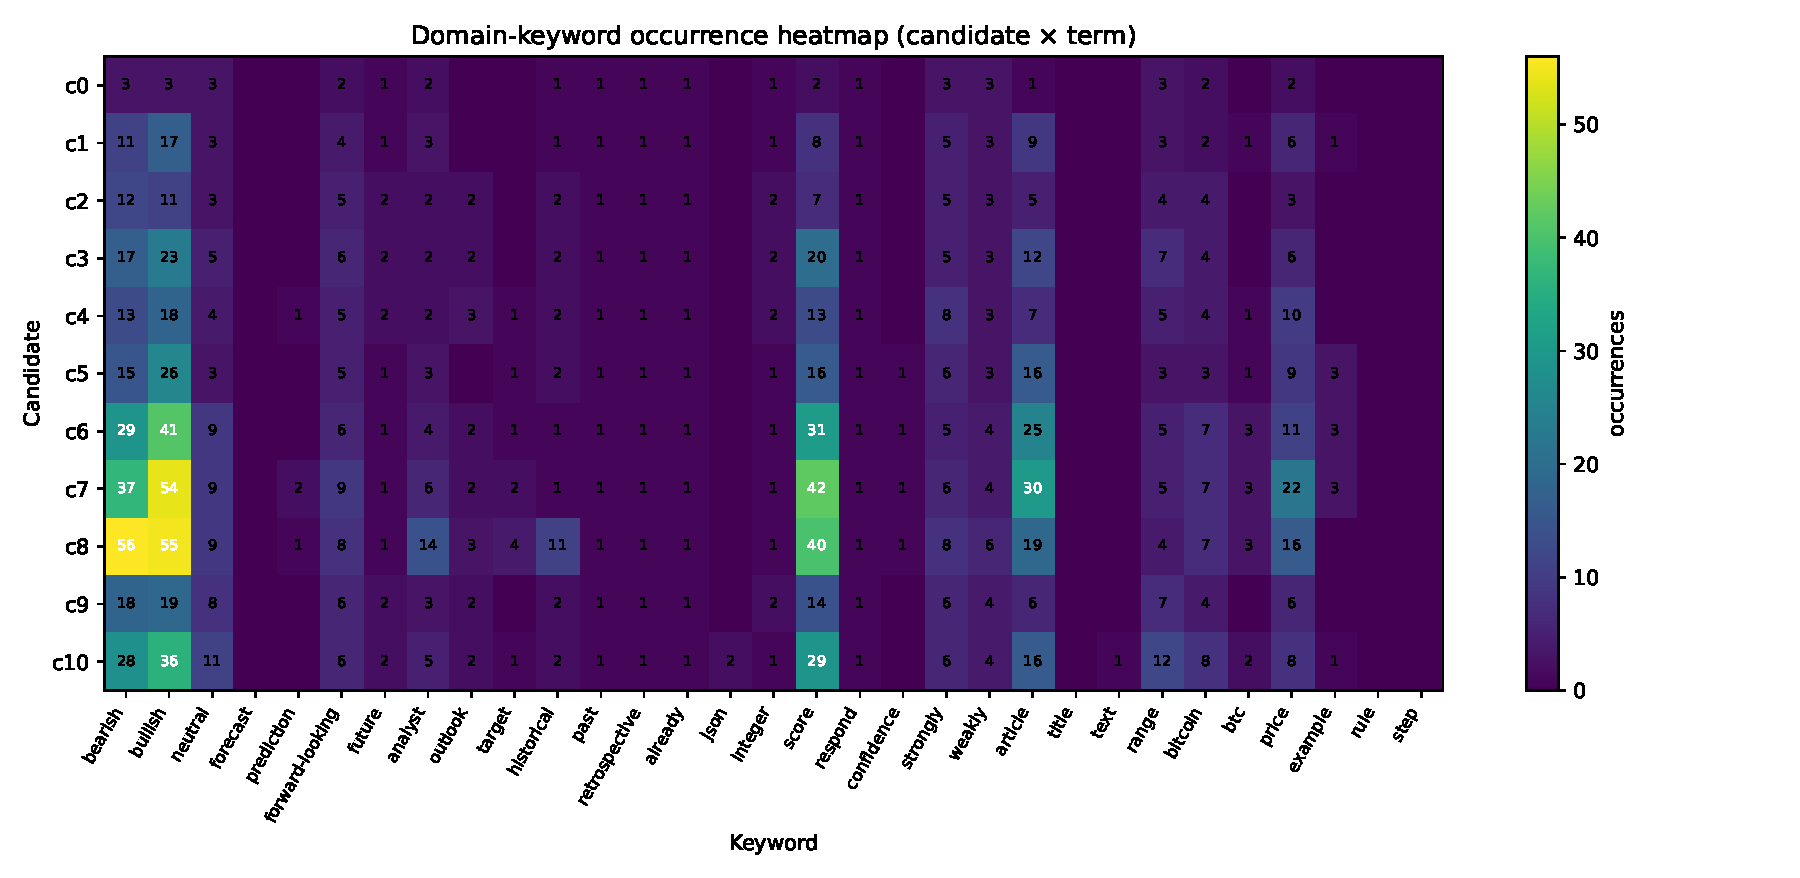
\includegraphics[width=\linewidth]{keyword_heatmap_claude_sonnet46.pdf}
    \end{minipage}
    \hfill
    \begin{minipage}{0.48\textwidth}
        \centering
        \textbf{GPT-OSS 120B}\\[0.2em]
        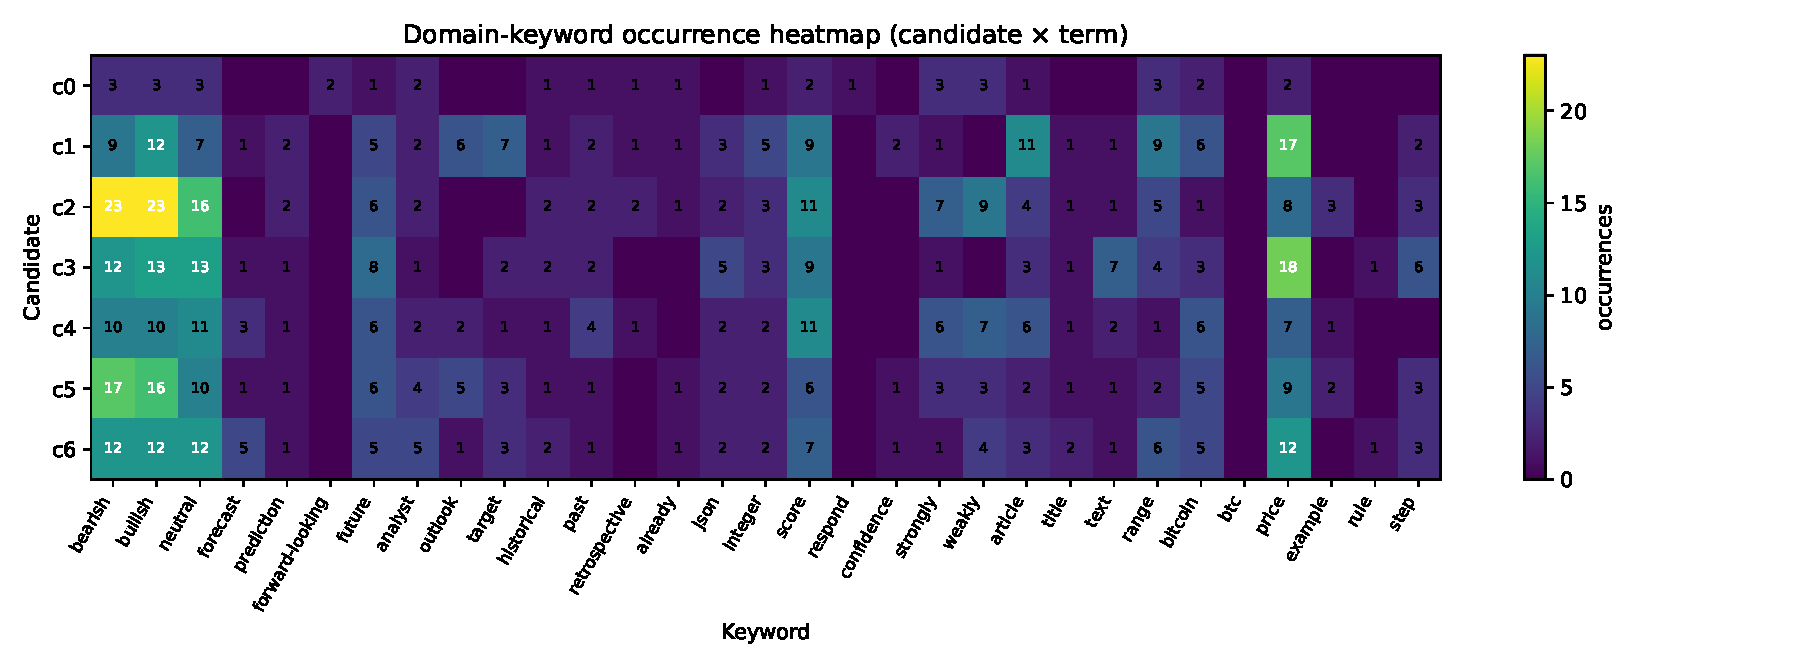
\includegraphics[width=\linewidth]{keyword_heatmap_gptoss120b.pdf}
    \end{minipage}

    \vspace{1em} % Adds vertical spacing between the rows

    % --- Row 2 ---
    \begin{minipage}{0.48\textwidth}
        \centering
        \textbf{Qwen 3.6}\\[0.2em]
        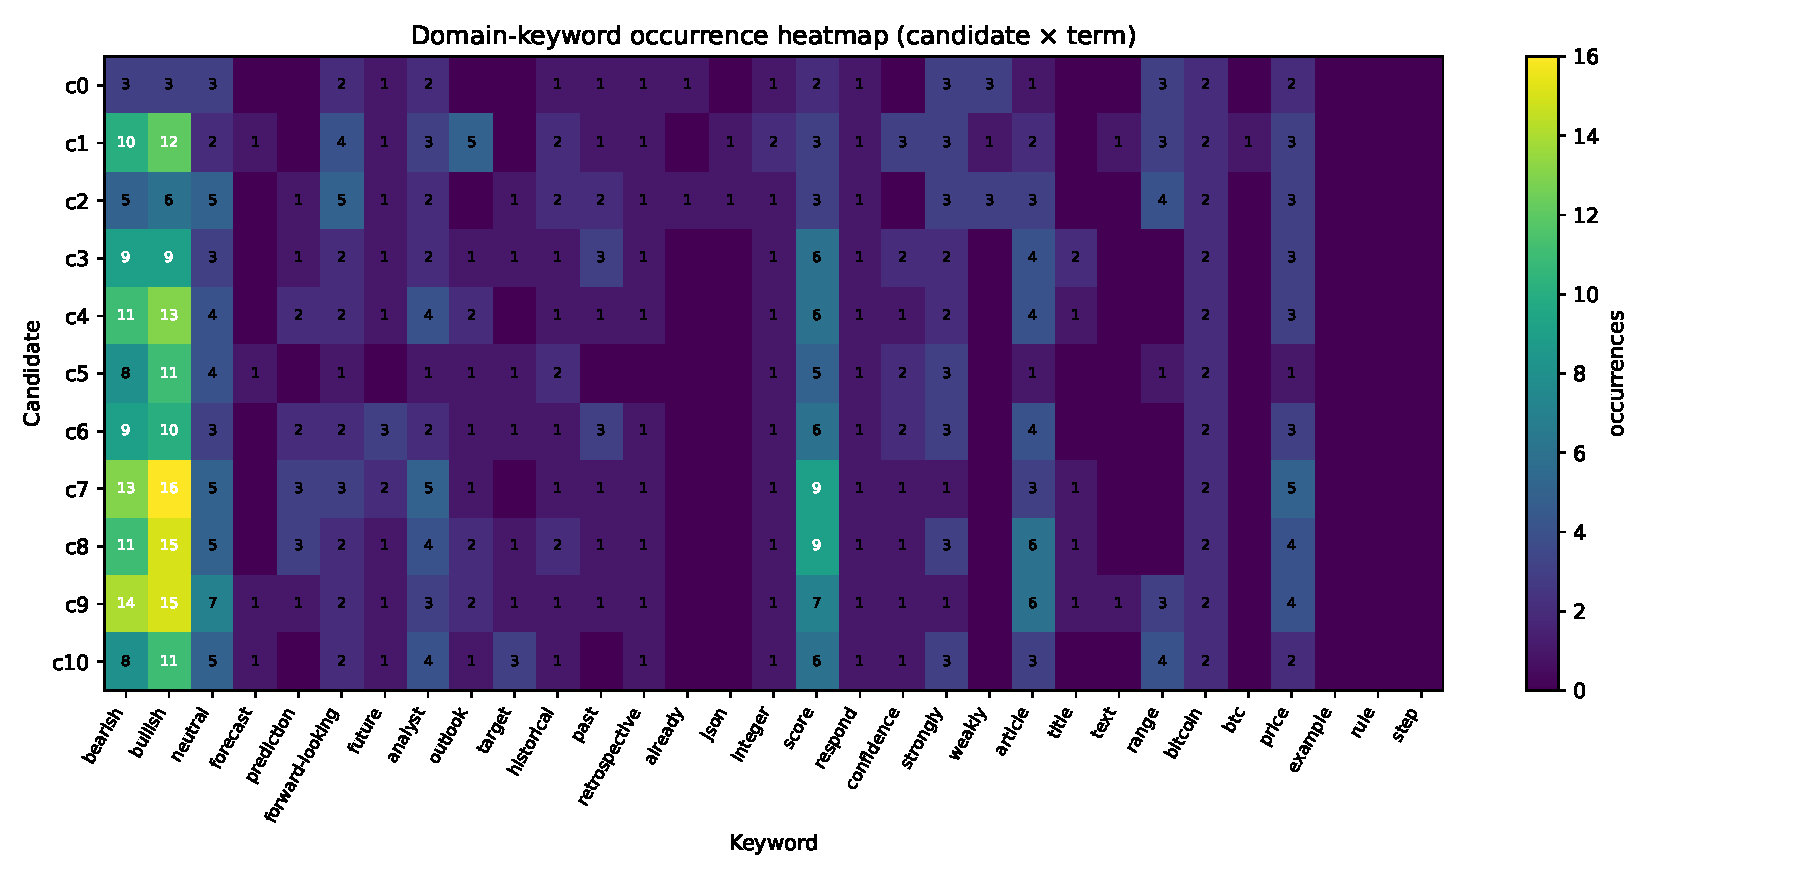
\includegraphics[width=\linewidth]{keyword_heatmap_qwen36.pdf}
    \end{minipage}
    \hfill
    \begin{minipage}{0.48\textwidth}
        \centering
        \textbf{Gemma 4 E2B}\\[0.2em]
        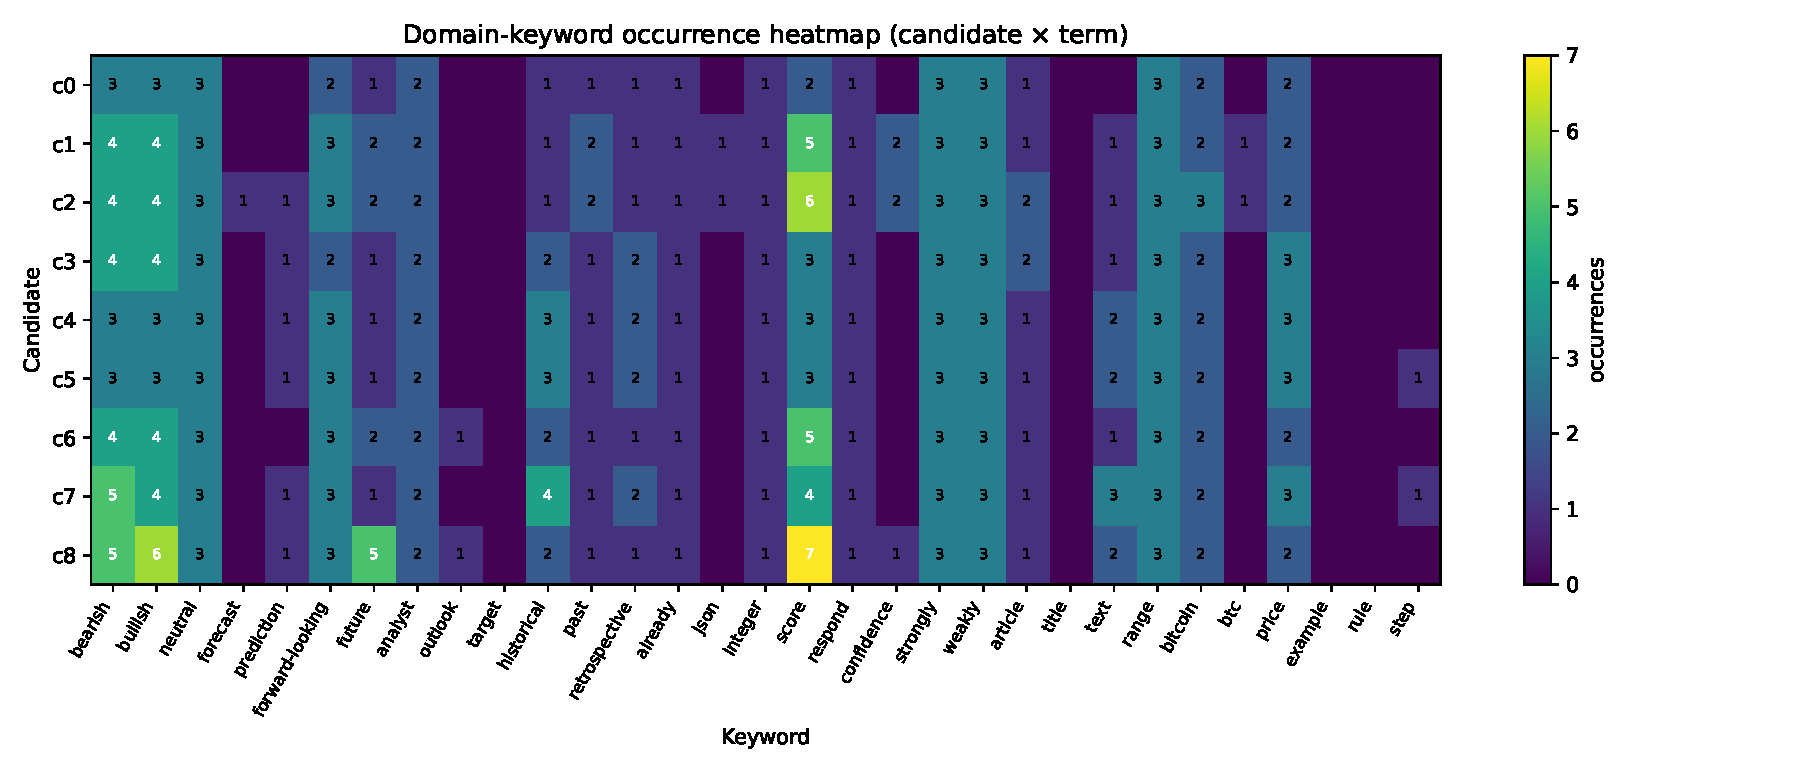
\includegraphics[width=\linewidth]{keyword_heatmap_gemma4e2b.pdf}
    \end{minipage}

    \caption{Domain-keyword heatmaps for the four GEPA source-model runs. Each heatmap summarizes how often Bitcoin-specific and prediction-specific vocabulary appears across the prompt candidates in that run.}
    \label{fig:keyword_heatmaps_appendix}
\end{figure*}


\bibliographystyle{ACM-Reference-Format}
\bibliography{references}

\end{document}